\documentclass[1p]{elsarticle_modified}
%\bibliographystyle{elsarticle-num}

%\usepackage[colorlinks]{hyperref}
%\usepackage{abbrmath_seonhwa} %\Abb, \Ascr, \Acal ,\Abf, \Afrak
\usepackage{amsfonts}
\usepackage{amssymb}
\usepackage{amsmath}
\usepackage{amsthm}
\usepackage{scalefnt}
\usepackage{amsbsy}
\usepackage{kotex}
\usepackage{caption}
\usepackage{subfig}
\usepackage{color}
\usepackage{graphicx}
\usepackage{xcolor} %% white, black, red, green, blue, cyan, magenta, yellow
\usepackage{float}
\usepackage{setspace}
\usepackage{hyperref}

\usepackage{tikz}
\usetikzlibrary{arrows}

\usepackage{multirow}
\usepackage{array} % fixed length table
\usepackage{hhline}

%%%%%%%%%%%%%%%%%%%%%
\makeatletter
\renewcommand*\env@matrix[1][\arraystretch]{%
	\edef\arraystretch{#1}%
	\hskip -\arraycolsep
	\let\@ifnextchar\new@ifnextchar
	\array{*\c@MaxMatrixCols c}}
\makeatother %https://tex.stackexchange.com/questions/14071/how-can-i-increase-the-line-spacing-in-a-matrix
%%%%%%%%%%%%%%%

\usepackage[normalem]{ulem}

\newcommand{\msout}[1]{\ifmmode\text{\sout{\ensuremath{#1}}}\else\sout{#1}\fi}
%SOURCE: \msout is \stkout macro in https://tex.stackexchange.com/questions/20609/strikeout-in-math-mode

\newcommand{\cancel}[1]{
	\ifmmode
	{\color{red}\msout{#1}}
	\else
	{\color{red}\sout{#1}}
	\fi
}

\newcommand{\add}[1]{
	{\color{blue}\uwave{#1}}
}

\newcommand{\replace}[2]{
	\ifmmode
	{\color{red}\msout{#1}}{\color{blue}\uwave{#2}}
	\else
	{\color{red}\sout{#1}}{\color{blue}\uwave{#2}}
	\fi
}

\newcommand{\Sol}{\mathcal{S}} %segment
\newcommand{\D}{D} %diagram
\newcommand{\A}{\mathcal{A}} %arc


%%%%%%%%%%%%%%%%%%%%%%%%%%%%%5 test

\def\sl{\operatorname{\textup{SL}}(2,\Cbb)}
\def\psl{\operatorname{\textup{PSL}}(2,\Cbb)}
\def\quan{\mkern 1mu \triangleright \mkern 1mu}

\theoremstyle{definition}
\newtheorem{thm}{Theorem}[section]
\newtheorem{prop}[thm]{Proposition}
\newtheorem{lem}[thm]{Lemma}
\newtheorem{ques}[thm]{Question}
\newtheorem{cor}[thm]{Corollary}
\newtheorem{defn}[thm]{Definition}
\newtheorem{exam}[thm]{Example}
\newtheorem{rmk}[thm]{Remark}
\newtheorem{alg}[thm]{Algorithm}

\newcommand{\I}{\sqrt{-1}}
\begin{document}

%\begin{frontmatter}
%
%\title{Boundary parabolic representations of knots up to 8 crossings}
%
%%% Group authors per affiliation:
%\author{Yunhi Cho} 
%\address{Department of Mathematics, University of Seoul, Seoul, Korea}
%\ead{yhcho@uos.ac.kr}
%
%
%\author{Seonhwa Kim} %\fnref{s_kim}}
%\address{Center for Geometry and Physics, Institute for Basic Science, Pohang, 37673, Korea}
%\ead{ryeona17@ibs.re.kr}
%
%\author{Hyuk Kim}
%\address{Department of Mathematical Sciences, Seoul National University, Seoul 08826, Korea}
%\ead{hyukkim@snu.ac.kr}
%
%\author{Seokbeom Yoon}
%\address{Department of Mathematical Sciences, Seoul National University, Seoul, 08826,  Korea}
%\ead{sbyoon15@snu.ac.kr}
%
%\begin{abstract}
%We find all boundary parabolic representation of knots up to 8 crossings.
%
%\end{abstract}
%\begin{keyword}
%    \MSC[2010] 57M25 
%\end{keyword}
%
%\end{frontmatter}

%\linenumbers
%\tableofcontents
%
\newcommand\colored[1]{\textcolor{white}{\rule[-0.35ex]{0.8em}{1.4ex}}\kern-0.8em\color{red} #1}%
%\newcommand\colored[1]{\textcolor{white}{ #1}\kern-2.17ex	\textcolor{white}{ #1}\kern-1.81ex	\textcolor{white}{ #1}\kern-2.15ex\color{red}#1	}

{\Large $\underline{12a_{0672}~(K12a_{0672})}$}

\setlength{\tabcolsep}{10pt}
\renewcommand{\arraystretch}{1.6}
\vspace{1cm}\begin{tabular}{m{100pt}>{\centering\arraybackslash}m{274pt}}
\multirow{5}{120pt}{
	\centering
	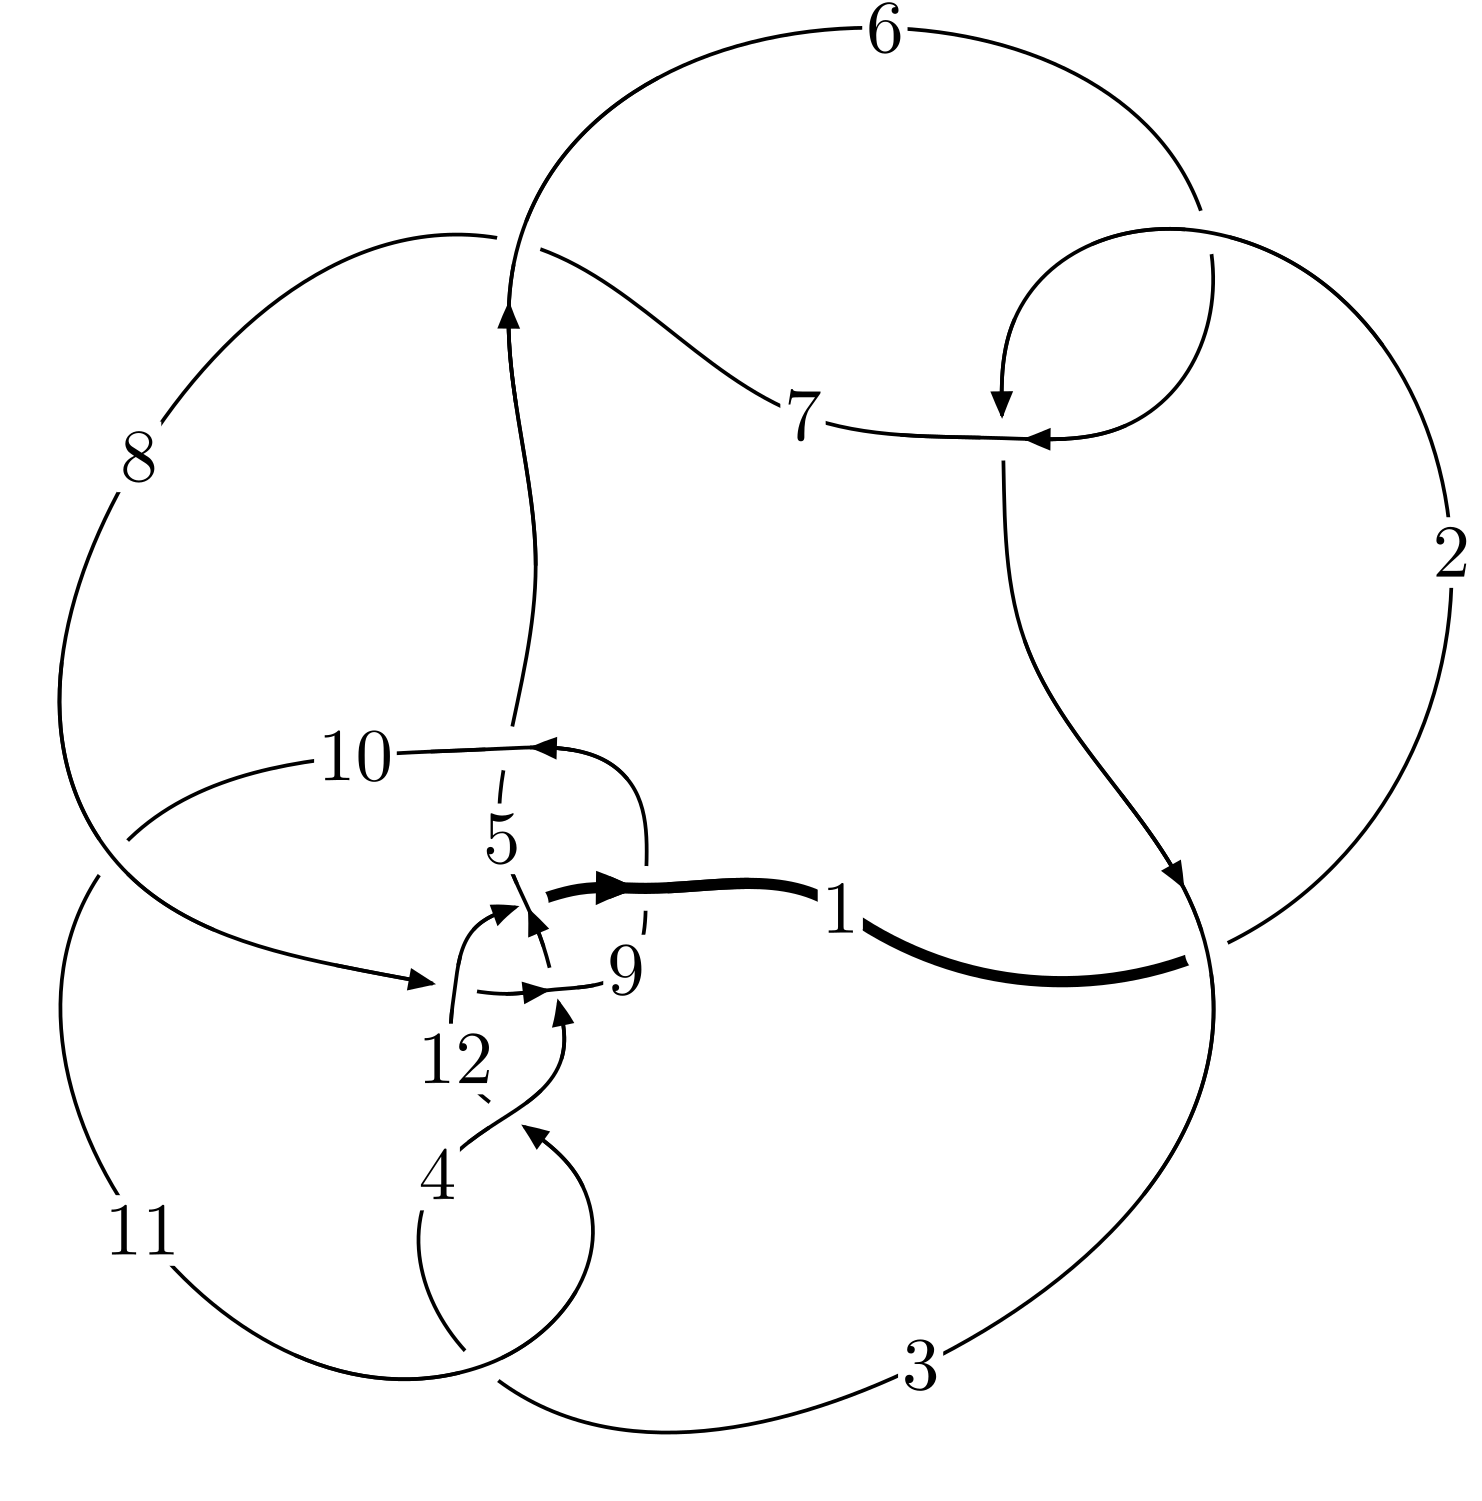
\includegraphics[width=112pt]{../../../GIT/diagram.site/Diagrams/png/1473_12a_0672.png}\\
\ \ \ A knot diagram\footnotemark}&
\allowdisplaybreaks
\textbf{Linearized knot diagam} \\
\cline{2-2}
 &
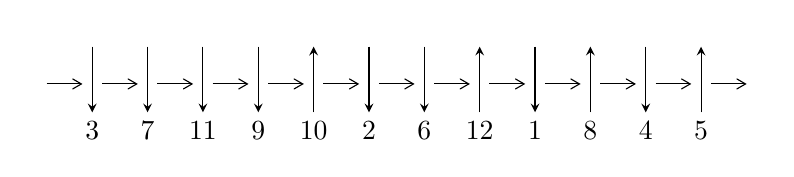
\begin{tikzpicture}[x=20pt, y=17pt]
	% nodes
	\node (C0) at (0, 0) {};
	\node (C1) at (1, 0) {};
	\node (C1U) at (1, +1) {};
	\node (C1D) at (1, -1) {3};

	\node (C2) at (2, 0) {};
	\node (C2U) at (2, +1) {};
	\node (C2D) at (2, -1) {7};

	\node (C3) at (3, 0) {};
	\node (C3U) at (3, +1) {};
	\node (C3D) at (3, -1) {11};

	\node (C4) at (4, 0) {};
	\node (C4U) at (4, +1) {};
	\node (C4D) at (4, -1) {9};

	\node (C5) at (5, 0) {};
	\node (C5U) at (5, +1) {};
	\node (C5D) at (5, -1) {10};

	\node (C6) at (6, 0) {};
	\node (C6U) at (6, +1) {};
	\node (C6D) at (6, -1) {2};

	\node (C7) at (7, 0) {};
	\node (C7U) at (7, +1) {};
	\node (C7D) at (7, -1) {6};

	\node (C8) at (8, 0) {};
	\node (C8U) at (8, +1) {};
	\node (C8D) at (8, -1) {12};

	\node (C9) at (9, 0) {};
	\node (C9U) at (9, +1) {};
	\node (C9D) at (9, -1) {1};

	\node (C10) at (10, 0) {};
	\node (C10U) at (10, +1) {};
	\node (C10D) at (10, -1) {8};

	\node (C11) at (11, 0) {};
	\node (C11U) at (11, +1) {};
	\node (C11D) at (11, -1) {4};

	\node (C12) at (12, 0) {};
	\node (C12U) at (12, +1) {};
	\node (C12D) at (12, -1) {5};
	\node (C13) at (13, 0) {};

	% arrows
	\draw[->,>={angle 60}]
	(C0) edge (C1) (C1) edge (C2) (C2) edge (C3) (C3) edge (C4) (C4) edge (C5) (C5) edge (C6) (C6) edge (C7) (C7) edge (C8) (C8) edge (C9) (C9) edge (C10) (C10) edge (C11) (C11) edge (C12) (C12) edge (C13) ;	\draw[->,>=stealth]
	(C1U) edge (C1D) (C2U) edge (C2D) (C3U) edge (C3D) (C4U) edge (C4D) (C5D) edge (C5U) (C6U) edge (C6D) (C7U) edge (C7D) (C8D) edge (C8U) (C9U) edge (C9D) (C10D) edge (C10U) (C11U) edge (C11D) (C12D) edge (C12U) ;
	\end{tikzpicture} \\
\hhline{~~} \\& 
\textbf{Solving Sequence} \\ \cline{2-2} 
 &
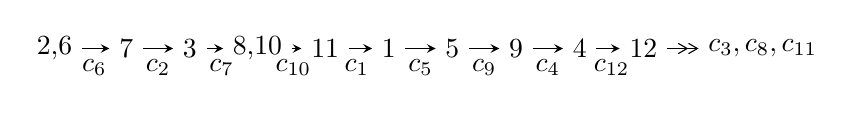
\begin{tikzpicture}[x=23pt, y=7pt]
	% node
	\node (A0) at (-1/8, 0) {2,6};
	\node (A1) at (1, 0) {7};
	\node (A2) at (2, 0) {3};
	\node (A3) at (49/16, 0) {8,10};
	\node (A4) at (33/8, 0) {11};
	\node (A5) at (41/8, 0) {1};
	\node (A6) at (49/8, 0) {5};
	\node (A7) at (57/8, 0) {9};
	\node (A8) at (65/8, 0) {4};
	\node (A9) at (73/8, 0) {12};
	\node (C1) at (1/2, -1) {$c_{6}$};
	\node (C2) at (3/2, -1) {$c_{2}$};
	\node (C3) at (5/2, -1) {$c_{7}$};
	\node (C4) at (29/8, -1) {$c_{10}$};
	\node (C5) at (37/8, -1) {$c_{1}$};
	\node (C6) at (45/8, -1) {$c_{5}$};
	\node (C7) at (53/8, -1) {$c_{9}$};
	\node (C8) at (61/8, -1) {$c_{4}$};
	\node (C9) at (69/8, -1) {$c_{12}$};
	\node (A10) at (11, 0) {$c_{3},c_{8},c_{11}$};

	% edge
	\draw[->,>=stealth]	
	(A0) edge (A1) (A1) edge (A2) (A2) edge (A3) (A3) edge (A4) (A4) edge (A5) (A5) edge (A6) (A6) edge (A7) (A7) edge (A8) (A8) edge (A9) ;
	\draw[->>,>={angle 60}]	
	(A9) edge (A10);
\end{tikzpicture} \\ 

\end{tabular} \\

\footnotetext{
The image of knot diagram is generated by the software ``\textbf{Draw programme}" developed by Andrew Bartholomew(\url{http://www.layer8.co.uk/maths/draw/index.htm\#Running-draw}), where we modified some parts for our purpose(\url{https://github.com/CATsTAILs/LinksPainter}).
}\phantom \\ \newline 
\centering \textbf{Ideals for irreducible components\footnotemark of $X_{\text{par}}$} 
 
\begin{align*}
I^u_{1}&=\langle 
-1.12902\times10^{190} u^{139}+9.34933\times10^{189} u^{138}+\cdots+1.58755\times10^{189} b-1.09247\times10^{190},\\
\phantom{I^u_{1}}&\phantom{= \langle  }3.44317\times10^{189} u^{139}-4.78461\times10^{189} u^{138}+\cdots+1.58755\times10^{189} a+2.42089\times10^{189},\\
\phantom{I^u_{1}}&\phantom{= \langle  }u^{140}-23 u^{138}+\cdots+3 u+1\rangle \\
I^u_{2}&=\langle 
2 u^{26}-9 u^{24}+\cdots+b+1,\;-7 u^{26}+2 u^{25}+\cdots+a-5,\;u^{27}-5 u^{25}+\cdots+2 u+1\rangle \\
I^u_{3}&=\langle 
- u^2+b,\;a-1,\;u^9- u^7+u^5- u-1\rangle \\
I^u_{4}&=\langle 
b-1,\;a-1,\;u+1\rangle \\
\\
\end{align*}
\raggedright * 4 irreducible components of $\dim_{\mathbb{C}}=0$, with total 177 representations.\\
\footnotetext{All coefficients of polynomials are rational numbers. But the coefficients are sometimes approximated in decimal forms when there is not enough margin.}
\newpage
\renewcommand{\arraystretch}{1}
\centering \section*{I. $I^u_{1}= \langle -1.13\times10^{190} u^{139}+9.35\times10^{189} u^{138}+\cdots+1.59\times10^{189} b-1.09\times10^{190},\;3.44\times10^{189} u^{139}-4.78\times10^{189} u^{138}+\cdots+1.59\times10^{189} a+2.42\times10^{189},\;u^{140}-23 u^{138}+\cdots+3 u+1 \rangle$}
\flushleft \textbf{(i) Arc colorings}\\
\begin{tabular}{m{7pt} m{180pt} m{7pt} m{180pt} }
\flushright $a_{2}=$&$\begin{pmatrix}0\\u\end{pmatrix}$ \\
\flushright $a_{6}=$&$\begin{pmatrix}1\\0\end{pmatrix}$ \\
\flushright $a_{7}=$&$\begin{pmatrix}1\\u^2\end{pmatrix}$ \\
\flushright $a_{3}=$&$\begin{pmatrix}- u\\- u^3+u\end{pmatrix}$ \\
\flushright $a_{8}=$&$\begin{pmatrix}- u^2+1\\u^2\end{pmatrix}$ \\
\flushright $a_{10}=$&$\begin{pmatrix}-2.16886 u^{139}+3.01383 u^{138}+\cdots+8.23078 u-1.52492\\7.11170 u^{139}-5.88917 u^{138}+\cdots+10.0353 u+6.88147\end{pmatrix}$ \\
\flushright $a_{11}=$&$\begin{pmatrix}-2.44142 u^{139}+0.866654 u^{138}+\cdots+5.48517 u-1.49467\\10.2142 u^{139}-7.71787 u^{138}+\cdots+19.1330 u+10.8573\end{pmatrix}$ \\
\flushright $a_{1}=$&$\begin{pmatrix}u^3\\u^5- u^3+u\end{pmatrix}$ \\
\flushright $a_{5}=$&$\begin{pmatrix}0.750500 u^{139}-1.39779 u^{138}+\cdots-3.01121 u+1.60235\\-10.5023 u^{139}+8.41153 u^{138}+\cdots-14.6571 u-11.6073\end{pmatrix}$ \\
\flushright $a_{9}=$&$\begin{pmatrix}0.943249 u^{139}-1.67414 u^{138}+\cdots+18.2542 u+3.74345\\12.1315 u^{139}-8.89990 u^{138}+\cdots+19.8046 u+11.8666\end{pmatrix}$ \\
\flushright $a_{4}=$&$\begin{pmatrix}-0.673830 u^{139}+0.601372 u^{138}+\cdots-14.0653 u+1.43963\\-12.6642 u^{139}+10.6942 u^{138}+\cdots-26.6036 u-15.5682\end{pmatrix}$ \\
\flushright $a_{12}=$&$\begin{pmatrix}5.96244 u^{139}+1.79950 u^{138}+\cdots-1.90249 u-2.91637\\12.5060 u^{139}-17.4576 u^{138}+\cdots+33.8666 u+16.1824\end{pmatrix}$\\&\end{tabular}
\flushleft \textbf{(ii) Obstruction class $= -1$}\\~\\
\flushleft \textbf{(iii) Cusp Shapes $= -24.6097 u^{139}+19.1757 u^{138}+\cdots-68.5270 u-30.0952$}\\~\\
\newpage\renewcommand{\arraystretch}{1}
\flushleft \textbf{(iv) u-Polynomials at the component}\newline \\
\begin{tabular}{m{50pt}|m{274pt}}
Crossings & \hspace{64pt}u-Polynomials at each crossing \\
\hline $$\begin{aligned}c_{1},c_{7}\end{aligned}$$&$\begin{aligned}
&u^{140}+46 u^{139}+\cdots+27 u+1
\end{aligned}$\\
\hline $$\begin{aligned}c_{2},c_{6}\end{aligned}$$&$\begin{aligned}
&u^{140}-23 u^{138}+\cdots+3 u+1
\end{aligned}$\\
\hline $$\begin{aligned}c_{3},c_{11}\end{aligned}$$&$\begin{aligned}
&u^{140}-6 u^{139}+\cdots-52600 u-21104
\end{aligned}$\\
\hline $$\begin{aligned}c_{4}\end{aligned}$$&$\begin{aligned}
&u^{140}+5 u^{139}+\cdots+35297 u-7759
\end{aligned}$\\
\hline $$\begin{aligned}c_{5}\end{aligned}$$&$\begin{aligned}
&u^{140}+u^{139}+\cdots+8346945 u+492823
\end{aligned}$\\
\hline $$\begin{aligned}c_{8}\end{aligned}$$&$\begin{aligned}
&u^{140}+u^{139}+\cdots-30 u-1
\end{aligned}$\\
\hline $$\begin{aligned}c_{9}\end{aligned}$$&$\begin{aligned}
&u^{140}+4 u^{139}+\cdots-49356 u+1718
\end{aligned}$\\
\hline $$\begin{aligned}c_{10}\end{aligned}$$&$\begin{aligned}
&u^{140}-6 u^{139}+\cdots+378931 u-19471
\end{aligned}$\\
\hline $$\begin{aligned}c_{12}\end{aligned}$$&$\begin{aligned}
&u^{140}-5 u^{138}+\cdots-39 u+1
\end{aligned}$\\
\hline
\end{tabular}\\~\\
\newpage\renewcommand{\arraystretch}{1}
\flushleft \textbf{(v) Riley Polynomials at the component}\newline \\
\begin{tabular}{m{50pt}|m{274pt}}
Crossings & \hspace{64pt}Riley Polynomials at each crossing \\
\hline $$\begin{aligned}c_{1},c_{7}\end{aligned}$$&$\begin{aligned}
&y^{140}+110 y^{139}+\cdots-551 y+1
\end{aligned}$\\
\hline $$\begin{aligned}c_{2},c_{6}\end{aligned}$$&$\begin{aligned}
&y^{140}-46 y^{139}+\cdots-27 y+1
\end{aligned}$\\
\hline $$\begin{aligned}c_{3},c_{11}\end{aligned}$$&$\begin{aligned}
&y^{140}-90 y^{139}+\cdots-46338922560 y+445378816
\end{aligned}$\\
\hline $$\begin{aligned}c_{4}\end{aligned}$$&$\begin{aligned}
&y^{140}-27 y^{139}+\cdots-3984913835 y+60202081
\end{aligned}$\\
\hline $$\begin{aligned}c_{5}\end{aligned}$$&$\begin{aligned}
&y^{140}-35 y^{139}+\cdots-12584572781083 y+242874509329
\end{aligned}$\\
\hline $$\begin{aligned}c_{8}\end{aligned}$$&$\begin{aligned}
&y^{140}+17 y^{139}+\cdots-82 y+1
\end{aligned}$\\
\hline $$\begin{aligned}c_{9}\end{aligned}$$&$\begin{aligned}
&y^{140}+4 y^{139}+\cdots-573798944 y+2951524
\end{aligned}$\\
\hline $$\begin{aligned}c_{10}\end{aligned}$$&$\begin{aligned}
&y^{140}-10 y^{139}+\cdots-105927544083 y+379119841
\end{aligned}$\\
\hline $$\begin{aligned}c_{12}\end{aligned}$$&$\begin{aligned}
&y^{140}-10 y^{139}+\cdots-447 y+1
\end{aligned}$\\
\hline
\end{tabular}\\~\\
\newpage\flushleft \textbf{(vi) Complex Volumes and Cusp Shapes}
$$\begin{array}{c|c|c}  
\text{Solutions to }I^u_{1}& \I (\text{vol} + \sqrt{-1}CS) & \text{Cusp shape}\\
 \hline 
\begin{aligned}
u &= -0.637272 + 0.774252 I \\
a &= \phantom{-}1.259990 - 0.002369 I \\
b &= -1.46338 + 0.19143 I\end{aligned}
 & \phantom{-}4.03902 - 0.85594 I & \phantom{-0.000000 } 0 \\ \hline\begin{aligned}
u &= -0.637272 - 0.774252 I \\
a &= \phantom{-}1.259990 + 0.002369 I \\
b &= -1.46338 - 0.19143 I\end{aligned}
 & \phantom{-}4.03902 + 0.85594 I & \phantom{-0.000000 } 0 \\ \hline\begin{aligned}
u &= \phantom{-}1.011350 + 0.012085 I \\
a &= -0.793113 + 0.223949 I \\
b &= \phantom{-}0.434213 + 0.174661 I\end{aligned}
 & -6.37978 + 0.00238 I & \phantom{-0.000000 } 0 \\ \hline\begin{aligned}
u &= \phantom{-}1.011350 - 0.012085 I \\
a &= -0.793113 - 0.223949 I \\
b &= \phantom{-}0.434213 - 0.174661 I\end{aligned}
 & -6.37978 - 0.00238 I & \phantom{-0.000000 } 0 \\ \hline\begin{aligned}
u &= \phantom{-}1.02392\phantom{ +0.000000I} \\
a &= -0.662890\phantom{ +0.000000I} \\
b &= \phantom{-}0.547273\phantom{ +0.000000I}\end{aligned}
 & -6.37988\phantom{ +0.000000I} & \phantom{-0.000000 } 0 \\ \hline\begin{aligned}
u &= \phantom{-}1.017280 + 0.184941 I \\
a &= -0.10014 - 1.71881 I \\
b &= \phantom{-}0.907707 - 1.026470 I\end{aligned}
 & -2.61394 - 5.50337 I & \phantom{-0.000000 } 0 \\ \hline\begin{aligned}
u &= \phantom{-}1.017280 - 0.184941 I \\
a &= -0.10014 + 1.71881 I \\
b &= \phantom{-}0.907707 + 1.026470 I\end{aligned}
 & -2.61394 + 5.50337 I & \phantom{-0.000000 } 0 \\ \hline\begin{aligned}
u &= \phantom{-}0.960574 + 0.067275 I \\
a &= \phantom{-}0.031287 - 1.341240 I \\
b &= -0.77872 - 1.36857 I\end{aligned}
 & -6.79916 - 5.81167 I & \phantom{-0.000000 } 0 \\ \hline\begin{aligned}
u &= \phantom{-}0.960574 - 0.067275 I \\
a &= \phantom{-}0.031287 + 1.341240 I \\
b &= -0.77872 + 1.36857 I\end{aligned}
 & -6.79916 + 5.81167 I & \phantom{-0.000000 } 0 \\ \hline\begin{aligned}
u &= \phantom{-}0.935095 + 0.212379 I \\
a &= -0.99923 - 1.11674 I \\
b &= \phantom{-}0.609100 - 0.820049 I\end{aligned}
 & -2.75766 - 3.86610 I & \phantom{-0.000000 } 0\\
 \hline 
 \end{array}$$\newpage$$\begin{array}{c|c|c}  
\text{Solutions to }I^u_{1}& \I (\text{vol} + \sqrt{-1}CS) & \text{Cusp shape}\\
 \hline 
\begin{aligned}
u &= \phantom{-}0.935095 - 0.212379 I \\
a &= -0.99923 + 1.11674 I \\
b &= \phantom{-}0.609100 + 0.820049 I\end{aligned}
 & -2.75766 + 3.86610 I & \phantom{-0.000000 } 0 \\ \hline\begin{aligned}
u &= -0.745262 + 0.727310 I \\
a &= -1.32678 - 1.06529 I \\
b &= \phantom{-}0.29285 + 1.73891 I\end{aligned}
 & -1.53936 - 5.19280 I & \phantom{-0.000000 } 0 \\ \hline\begin{aligned}
u &= -0.745262 - 0.727310 I \\
a &= -1.32678 + 1.06529 I \\
b &= \phantom{-}0.29285 - 1.73891 I\end{aligned}
 & -1.53936 + 5.19280 I & \phantom{-0.000000 } 0 \\ \hline\begin{aligned}
u &= -0.879911 + 0.561119 I \\
a &= -1.44299 + 1.54598 I \\
b &= \phantom{-}0.932754 - 0.266761 I\end{aligned}
 & -3.48917 + 5.68868 I & \phantom{-0.000000 } 0 \\ \hline\begin{aligned}
u &= -0.879911 - 0.561119 I \\
a &= -1.44299 - 1.54598 I \\
b &= \phantom{-}0.932754 + 0.266761 I\end{aligned}
 & -3.48917 - 5.68868 I & \phantom{-0.000000 } 0 \\ \hline\begin{aligned}
u &= -0.942327 + 0.122868 I \\
a &= \phantom{-}0.449286 + 1.238000 I \\
b &= \phantom{-}1.21615 + 0.87500 I\end{aligned}
 & -0.41690 + 1.63156 I & \phantom{-0.000000 } 0 \\ \hline\begin{aligned}
u &= -0.942327 - 0.122868 I \\
a &= \phantom{-}0.449286 - 1.238000 I \\
b &= \phantom{-}1.21615 - 0.87500 I\end{aligned}
 & -0.41690 - 1.63156 I & \phantom{-0.000000 } 0 \\ \hline\begin{aligned}
u &= \phantom{-}0.779383 + 0.703759 I \\
a &= \phantom{-}0.594080 + 0.164147 I \\
b &= -0.284029 + 1.298440 I\end{aligned}
 & -1.17235 - 5.37475 I & \phantom{-0.000000 } 0 \\ \hline\begin{aligned}
u &= \phantom{-}0.779383 - 0.703759 I \\
a &= \phantom{-}0.594080 - 0.164147 I \\
b &= -0.284029 - 1.298440 I\end{aligned}
 & -1.17235 + 5.37475 I & \phantom{-0.000000 } 0 \\ \hline\begin{aligned}
u &= \phantom{-}1.028920 + 0.260799 I \\
a &= \phantom{-}0.202383 + 1.007000 I \\
b &= -1.027600 + 0.942415 I\end{aligned}
 & -0.71138 - 8.15105 I & \phantom{-0.000000 } 0\\
 \hline 
 \end{array}$$\newpage$$\begin{array}{c|c|c}  
\text{Solutions to }I^u_{1}& \I (\text{vol} + \sqrt{-1}CS) & \text{Cusp shape}\\
 \hline 
\begin{aligned}
u &= \phantom{-}1.028920 - 0.260799 I \\
a &= \phantom{-}0.202383 - 1.007000 I \\
b &= -1.027600 - 0.942415 I\end{aligned}
 & -0.71138 + 8.15105 I & \phantom{-0.000000 } 0 \\ \hline\begin{aligned}
u &= -0.698027 + 0.608519 I \\
a &= \phantom{-}1.240040 - 0.212448 I \\
b &= \phantom{-}0.202084 - 0.411980 I\end{aligned}
 & -1.78318 - 0.31648 I & \phantom{-0.000000 } 0 \\ \hline\begin{aligned}
u &= -0.698027 - 0.608519 I \\
a &= \phantom{-}1.240040 + 0.212448 I \\
b &= \phantom{-}0.202084 + 0.411980 I\end{aligned}
 & -1.78318 + 0.31648 I & \phantom{-0.000000 } 0 \\ \hline\begin{aligned}
u &= \phantom{-}0.814503 + 0.701975 I \\
a &= \phantom{-}2.26007 + 1.41025 I \\
b &= -0.482272 - 0.358926 I\end{aligned}
 & -1.59077 + 3.20105 I & \phantom{-0.000000 } 0 \\ \hline\begin{aligned}
u &= \phantom{-}0.814503 - 0.701975 I \\
a &= \phantom{-}2.26007 - 1.41025 I \\
b &= -0.482272 + 0.358926 I\end{aligned}
 & -1.59077 - 3.20105 I & \phantom{-0.000000 } 0 \\ \hline\begin{aligned}
u &= \phantom{-}0.753855 + 0.775047 I \\
a &= \phantom{-}1.95414 + 1.03664 I \\
b &= -1.76398 - 0.64520 I\end{aligned}
 & \phantom{-}5.39914 + 0.65450 I & \phantom{-0.000000 } 0 \\ \hline\begin{aligned}
u &= \phantom{-}0.753855 - 0.775047 I \\
a &= \phantom{-}1.95414 - 1.03664 I \\
b &= -1.76398 + 0.64520 I\end{aligned}
 & \phantom{-}5.39914 - 0.65450 I & \phantom{-0.000000 } 0 \\ \hline\begin{aligned}
u &= -1.056330 + 0.255019 I \\
a &= -0.736586 - 0.502673 I \\
b &= -0.521953 + 0.416676 I\end{aligned}
 & -0.81071 - 1.71202 I & \phantom{-0.000000 } 0 \\ \hline\begin{aligned}
u &= -1.056330 - 0.255019 I \\
a &= -0.736586 + 0.502673 I \\
b &= -0.521953 - 0.416676 I\end{aligned}
 & -0.81071 + 1.71202 I & \phantom{-0.000000 } 0 \\ \hline\begin{aligned}
u &= \phantom{-}0.867566 + 0.659942 I \\
a &= \phantom{-}0.92138 - 1.11949 I \\
b &= \phantom{-}0.201058 + 1.214890 I\end{aligned}
 & \phantom{-}2.14246 - 2.56378 I & \phantom{-0.000000 } 0\\
 \hline 
 \end{array}$$\newpage$$\begin{array}{c|c|c}  
\text{Solutions to }I^u_{1}& \I (\text{vol} + \sqrt{-1}CS) & \text{Cusp shape}\\
 \hline 
\begin{aligned}
u &= \phantom{-}0.867566 - 0.659942 I \\
a &= \phantom{-}0.92138 + 1.11949 I \\
b &= \phantom{-}0.201058 - 1.214890 I\end{aligned}
 & \phantom{-}2.14246 + 2.56378 I & \phantom{-0.000000 } 0 \\ \hline\begin{aligned}
u &= -0.842091 + 0.343705 I \\
a &= -0.82656 + 2.16593 I \\
b &= \phantom{-}0.502030 - 0.113865 I\end{aligned}
 & -3.58332 + 5.58428 I & \phantom{-0.000000 } 0 \\ \hline\begin{aligned}
u &= -0.842091 - 0.343705 I \\
a &= -0.82656 - 2.16593 I \\
b &= \phantom{-}0.502030 + 0.113865 I\end{aligned}
 & -3.58332 - 5.58428 I & \phantom{-0.000000 } 0 \\ \hline\begin{aligned}
u &= -0.723221 + 0.823322 I \\
a &= \phantom{-}1.37155 - 0.80169 I \\
b &= -1.24957 + 1.08257 I\end{aligned}
 & \phantom{-}4.04950 - 4.96120 I & \phantom{-0.000000 } 0 \\ \hline\begin{aligned}
u &= -0.723221 - 0.823322 I \\
a &= \phantom{-}1.37155 + 0.80169 I \\
b &= -1.24957 - 1.08257 I\end{aligned}
 & \phantom{-}4.04950 + 4.96120 I & \phantom{-0.000000 } 0 \\ \hline\begin{aligned}
u &= -0.903834 + 0.016154 I \\
a &= -1.16716 - 2.44769 I \\
b &= \phantom{-}0.474301 - 0.934610 I\end{aligned}
 & -5.80281 - 4.37403 I & \phantom{-0.000000 } 0 \\ \hline\begin{aligned}
u &= -0.903834 - 0.016154 I \\
a &= -1.16716 + 2.44769 I \\
b &= \phantom{-}0.474301 + 0.934610 I\end{aligned}
 & -5.80281 + 4.37403 I & \phantom{-0.000000 } 0 \\ \hline\begin{aligned}
u &= \phantom{-}0.825710 + 0.725196 I \\
a &= -2.37145 - 1.23965 I \\
b &= \phantom{-}1.49023 - 0.63141 I\end{aligned}
 & \phantom{-}0.76253 - 1.70916 I & \phantom{-0.000000 } 0 \\ \hline\begin{aligned}
u &= \phantom{-}0.825710 - 0.725196 I \\
a &= -2.37145 + 1.23965 I \\
b &= \phantom{-}1.49023 + 0.63141 I\end{aligned}
 & \phantom{-}0.76253 + 1.70916 I & \phantom{-0.000000 } 0 \\ \hline\begin{aligned}
u &= \phantom{-}0.755812 + 0.805461 I \\
a &= \phantom{-}1.51275 + 0.00873 I \\
b &= -1.239210 + 0.216436 I\end{aligned}
 & \phantom{-}4.70506 - 1.57922 I & \phantom{-0.000000 } 0\\
 \hline 
 \end{array}$$\newpage$$\begin{array}{c|c|c}  
\text{Solutions to }I^u_{1}& \I (\text{vol} + \sqrt{-1}CS) & \text{Cusp shape}\\
 \hline 
\begin{aligned}
u &= \phantom{-}0.755812 - 0.805461 I \\
a &= \phantom{-}1.51275 - 0.00873 I \\
b &= -1.239210 - 0.216436 I\end{aligned}
 & \phantom{-}4.70506 + 1.57922 I & \phantom{-0.000000 } 0 \\ \hline\begin{aligned}
u &= -0.909980 + 0.626719 I \\
a &= \phantom{-}2.59745 - 0.58433 I \\
b &= -1.086080 - 0.753826 I\end{aligned}
 & -3.72434 - 0.98515 I & \phantom{-0.000000 } 0 \\ \hline\begin{aligned}
u &= -0.909980 - 0.626719 I \\
a &= \phantom{-}2.59745 + 0.58433 I \\
b &= -1.086080 + 0.753826 I\end{aligned}
 & -3.72434 + 0.98515 I & \phantom{-0.000000 } 0 \\ \hline\begin{aligned}
u &= -0.682246 + 0.872598 I \\
a &= -0.819823 + 0.713190 I \\
b &= \phantom{-}0.988583 - 0.825638 I\end{aligned}
 & \phantom{-}0.32816 - 5.72400 I & \phantom{-0.000000 } 0 \\ \hline\begin{aligned}
u &= -0.682246 - 0.872598 I \\
a &= -0.819823 - 0.713190 I \\
b &= \phantom{-}0.988583 + 0.825638 I\end{aligned}
 & \phantom{-}0.32816 + 5.72400 I & \phantom{-0.000000 } 0 \\ \hline\begin{aligned}
u &= \phantom{-}0.688053 + 0.882581 I \\
a &= -1.51131 - 0.78456 I \\
b &= \phantom{-}1.41721 + 0.87490 I\end{aligned}
 & \phantom{-}1.92917 + 13.82410 I & \phantom{-0.000000 } 0 \\ \hline\begin{aligned}
u &= \phantom{-}0.688053 - 0.882581 I \\
a &= -1.51131 + 0.78456 I \\
b &= \phantom{-}1.41721 - 0.87490 I\end{aligned}
 & \phantom{-}1.92917 - 13.82410 I & \phantom{-0.000000 } 0 \\ \hline\begin{aligned}
u &= \phantom{-}0.869980 + 0.708482 I \\
a &= -2.43913 + 2.34344 I \\
b &= -0.01244 - 3.15134 I\end{aligned}
 & \phantom{-}0.81893 - 2.71443 I & \phantom{-0.000000 } 0 \\ \hline\begin{aligned}
u &= \phantom{-}0.869980 - 0.708482 I \\
a &= -2.43913 - 2.34344 I \\
b &= -0.01244 + 3.15134 I\end{aligned}
 & \phantom{-}0.81893 + 2.71443 I & \phantom{-0.000000 } 0 \\ \hline\begin{aligned}
u &= -0.743353 + 0.852323 I \\
a &= -1.53534 + 1.10594 I \\
b &= \phantom{-}1.52043 - 0.80465 I\end{aligned}
 & \phantom{-}6.56077 - 7.34720 I & \phantom{-0.000000 } 0\\
 \hline 
 \end{array}$$\newpage$$\begin{array}{c|c|c}  
\text{Solutions to }I^u_{1}& \I (\text{vol} + \sqrt{-1}CS) & \text{Cusp shape}\\
 \hline 
\begin{aligned}
u &= -0.743353 - 0.852323 I \\
a &= -1.53534 - 1.10594 I \\
b &= \phantom{-}1.52043 + 0.80465 I\end{aligned}
 & \phantom{-}6.56077 + 7.34720 I & \phantom{-0.000000 } 0 \\ \hline\begin{aligned}
u &= \phantom{-}0.808654 + 0.795047 I \\
a &= -0.84326 - 1.30185 I \\
b &= \phantom{-}1.14857 + 0.84874 I\end{aligned}
 & \phantom{-}3.37292 - 1.72822 I & \phantom{-0.000000 } 0 \\ \hline\begin{aligned}
u &= \phantom{-}0.808654 - 0.795047 I \\
a &= -0.84326 + 1.30185 I \\
b &= \phantom{-}1.14857 - 0.84874 I\end{aligned}
 & \phantom{-}3.37292 + 1.72822 I & \phantom{-0.000000 } 0 \\ \hline\begin{aligned}
u &= -0.778044 + 0.839237 I \\
a &= \phantom{-}1.48124 - 0.72700 I \\
b &= -0.995013 + 0.401193 I\end{aligned}
 & \phantom{-}3.97627 - 2.35525 I & \phantom{-0.000000 } 0 \\ \hline\begin{aligned}
u &= -0.778044 - 0.839237 I \\
a &= \phantom{-}1.48124 + 0.72700 I \\
b &= -0.995013 - 0.401193 I\end{aligned}
 & \phantom{-}3.97627 + 2.35525 I & \phantom{-0.000000 } 0 \\ \hline\begin{aligned}
u &= \phantom{-}0.755240 + 0.861550 I \\
a &= -0.744629 + 0.046044 I \\
b &= \phantom{-}0.857049 + 0.206186 I\end{aligned}
 & \phantom{-}6.69538 - 2.46683 I & \phantom{-0.000000 } 0 \\ \hline\begin{aligned}
u &= \phantom{-}0.755240 - 0.861550 I \\
a &= -0.744629 - 0.046044 I \\
b &= \phantom{-}0.857049 - 0.206186 I\end{aligned}
 & \phantom{-}6.69538 + 2.46683 I & \phantom{-0.000000 } 0 \\ \hline\begin{aligned}
u &= \phantom{-}0.681796 + 0.920876 I \\
a &= \phantom{-}1.37920 + 0.41022 I \\
b &= -1.135510 - 0.468563 I\end{aligned}
 & \phantom{-}1.77849 + 4.30367 I & \phantom{-0.000000 } 0 \\ \hline\begin{aligned}
u &= \phantom{-}0.681796 - 0.920876 I \\
a &= \phantom{-}1.37920 - 0.41022 I \\
b &= -1.135510 + 0.468563 I\end{aligned}
 & \phantom{-}1.77849 - 4.30367 I & \phantom{-0.000000 } 0 \\ \hline\begin{aligned}
u &= -0.826457 + 0.794325 I \\
a &= \phantom{-}1.202260 - 0.027016 I \\
b &= -0.984494 + 0.419369 I\end{aligned}
 & \phantom{-}6.94462 + 0.32347 I & \phantom{-0.000000 } 0\\
 \hline 
 \end{array}$$\newpage$$\begin{array}{c|c|c}  
\text{Solutions to }I^u_{1}& \I (\text{vol} + \sqrt{-1}CS) & \text{Cusp shape}\\
 \hline 
\begin{aligned}
u &= -0.826457 - 0.794325 I \\
a &= \phantom{-}1.202260 + 0.027016 I \\
b &= -0.984494 - 0.419369 I\end{aligned}
 & \phantom{-}6.94462 - 0.32347 I & \phantom{-0.000000 } 0 \\ \hline\begin{aligned}
u &= -0.852687\phantom{ +0.000000I} \\
a &= \phantom{-}0.457434\phantom{ +0.000000I} \\
b &= -1.66923\phantom{ +0.000000I}\end{aligned}
 & -3.61800\phantom{ +0.000000I} & \phantom{-0.000000 } 0 \\ \hline\begin{aligned}
u &= \phantom{-}0.917783 + 0.695410 I \\
a &= -2.86701 - 0.05432 I \\
b &= \phantom{-}0.606389 - 0.484552 I\end{aligned}
 & -1.91229 - 8.57330 I & \phantom{-0.000000 } 0 \\ \hline\begin{aligned}
u &= \phantom{-}0.917783 - 0.695410 I \\
a &= -2.86701 + 0.05432 I \\
b &= \phantom{-}0.606389 + 0.484552 I\end{aligned}
 & -1.91229 + 8.57330 I & \phantom{-0.000000 } 0 \\ \hline\begin{aligned}
u &= -1.134300 + 0.207590 I \\
a &= \phantom{-}0.096639 - 1.075190 I \\
b &= -1.14181 - 0.89648 I\end{aligned}
 & -5.4923 + 13.5525 I & \phantom{-0.000000 } 0 \\ \hline\begin{aligned}
u &= -1.134300 - 0.207590 I \\
a &= \phantom{-}0.096639 + 1.075190 I \\
b &= -1.14181 + 0.89648 I\end{aligned}
 & -5.4923 - 13.5525 I & \phantom{-0.000000 } 0 \\ \hline\begin{aligned}
u &= \phantom{-}0.780067 + 0.855177 I \\
a &= \phantom{-}1.169240 - 0.256613 I \\
b &= -0.748320 - 0.368537 I\end{aligned}
 & \phantom{-}3.80136 + 3.65097 I & \phantom{-0.000000 } 0 \\ \hline\begin{aligned}
u &= \phantom{-}0.780067 - 0.855177 I \\
a &= \phantom{-}1.169240 + 0.256613 I \\
b &= -0.748320 + 0.368537 I\end{aligned}
 & \phantom{-}3.80136 - 3.65097 I & \phantom{-0.000000 } 0 \\ \hline\begin{aligned}
u &= \phantom{-}0.911894 + 0.713790 I \\
a &= \phantom{-}1.56209 + 1.20005 I \\
b &= -1.66376 - 0.55939 I\end{aligned}
 & \phantom{-}0.49607 - 3.78910 I & \phantom{-0.000000 } 0 \\ \hline\begin{aligned}
u &= \phantom{-}0.911894 - 0.713790 I \\
a &= \phantom{-}1.56209 - 1.20005 I \\
b &= -1.66376 + 0.55939 I\end{aligned}
 & \phantom{-}0.49607 + 3.78910 I & \phantom{-0.000000 } 0\\
 \hline 
 \end{array}$$\newpage$$\begin{array}{c|c|c}  
\text{Solutions to }I^u_{1}& \I (\text{vol} + \sqrt{-1}CS) & \text{Cusp shape}\\
 \hline 
\begin{aligned}
u &= \phantom{-}1.142360 + 0.194064 I \\
a &= -0.021770 + 0.653476 I \\
b &= -0.548491 + 0.752756 I\end{aligned}
 & -6.96686 - 5.37463 I & \phantom{-0.000000 } 0 \\ \hline\begin{aligned}
u &= \phantom{-}1.142360 - 0.194064 I \\
a &= -0.021770 - 0.653476 I \\
b &= -0.548491 - 0.752756 I\end{aligned}
 & -6.96686 + 5.37463 I & \phantom{-0.000000 } 0 \\ \hline\begin{aligned}
u &= -0.961955 + 0.652383 I \\
a &= -0.720924 - 0.064504 I \\
b &= \phantom{-}0.122679 - 0.405902 I\end{aligned}
 & -2.55925 + 5.34694 I & \phantom{-0.000000 } 0 \\ \hline\begin{aligned}
u &= -0.961955 - 0.652383 I \\
a &= -0.720924 + 0.064504 I \\
b &= \phantom{-}0.122679 + 0.405902 I\end{aligned}
 & -2.55925 - 5.34694 I & \phantom{-0.000000 } 0 \\ \hline\begin{aligned}
u &= -0.821488 + 0.151520 I \\
a &= \phantom{-}0.88215 - 1.13546 I \\
b &= \phantom{-}0.01092 - 1.59339 I\end{aligned}
 & -2.39930 + 0.35910 I & \phantom{-0.000000 } 0 \\ \hline\begin{aligned}
u &= -0.821488 - 0.151520 I \\
a &= \phantom{-}0.88215 + 1.13546 I \\
b &= \phantom{-}0.01092 + 1.59339 I\end{aligned}
 & -2.39930 - 0.35910 I & \phantom{-0.000000 } 0 \\ \hline\begin{aligned}
u &= -0.956096 + 0.673027 I \\
a &= \phantom{-}0.253311 + 0.055704 I \\
b &= \phantom{-}0.150893 - 0.986242 I\end{aligned}
 & -2.29376 + 5.19888 I & \phantom{-0.000000 } 0 \\ \hline\begin{aligned}
u &= -0.956096 - 0.673027 I \\
a &= \phantom{-}0.253311 - 0.055704 I \\
b &= \phantom{-}0.150893 + 0.986242 I\end{aligned}
 & -2.29376 - 5.19888 I & \phantom{-0.000000 } 0 \\ \hline\begin{aligned}
u &= -0.220210 + 0.800606 I \\
a &= -0.382355 - 0.292702 I \\
b &= \phantom{-}0.598812 + 0.349617 I\end{aligned}
 & -2.39895 + 2.29733 I & \phantom{-0.000000 } 0 \\ \hline\begin{aligned}
u &= -0.220210 - 0.800606 I \\
a &= -0.382355 + 0.292702 I \\
b &= \phantom{-}0.598812 - 0.349617 I\end{aligned}
 & -2.39895 - 2.29733 I & \phantom{-0.000000 } 0\\
 \hline 
 \end{array}$$\newpage$$\begin{array}{c|c|c}  
\text{Solutions to }I^u_{1}& \I (\text{vol} + \sqrt{-1}CS) & \text{Cusp shape}\\
 \hline 
\begin{aligned}
u &= -0.822610\phantom{ +0.000000I} \\
a &= \phantom{-}0.318844\phantom{ +0.000000I} \\
b &= \phantom{-}0.502826\phantom{ +0.000000I}\end{aligned}
 & -1.19691\phantom{ +0.000000I} & \phantom{-0.000000 } 0 \\ \hline\begin{aligned}
u &= \phantom{-}0.152222 + 0.806909 I \\
a &= -1.214810 + 0.533344 I \\
b &= \phantom{-}1.119620 - 0.651030 I\end{aligned}
 & -1.13413 - 10.33050 I & \phantom{-0.000000 } 0 \\ \hline\begin{aligned}
u &= \phantom{-}0.152222 - 0.806909 I \\
a &= -1.214810 - 0.533344 I \\
b &= \phantom{-}1.119620 + 0.651030 I\end{aligned}
 & -1.13413 + 10.33050 I & \phantom{-0.000000 } 0 \\ \hline\begin{aligned}
u &= -0.960838 + 0.701466 I \\
a &= -1.20259 - 1.18921 I \\
b &= -0.47405 + 1.83054 I\end{aligned}
 & -2.19001 + 10.66420 I & \phantom{-0.000000 } 0 \\ \hline\begin{aligned}
u &= -0.960838 - 0.701466 I \\
a &= -1.20259 + 1.18921 I \\
b &= -0.47405 - 1.83054 I\end{aligned}
 & -2.19001 - 10.66420 I & \phantom{-0.000000 } 0 \\ \hline\begin{aligned}
u &= \phantom{-}1.118710 + 0.423282 I \\
a &= -0.540688 + 0.645565 I \\
b &= -0.875083 - 0.618712 I\end{aligned}
 & -4.20294 + 5.96067 I & \phantom{-0.000000 } 0 \\ \hline\begin{aligned}
u &= \phantom{-}1.118710 - 0.423282 I \\
a &= -0.540688 - 0.645565 I \\
b &= -0.875083 + 0.618712 I\end{aligned}
 & -4.20294 - 5.96067 I & \phantom{-0.000000 } 0 \\ \hline\begin{aligned}
u &= \phantom{-}0.762326 + 0.243629 I \\
a &= \phantom{-}0.54841 - 1.76335 I \\
b &= \phantom{-}0.458839 + 0.009570 I\end{aligned}
 & \phantom{-}0.95809 - 2.33250 I & \phantom{-0.000000 } 0 \\ \hline\begin{aligned}
u &= \phantom{-}0.762326 - 0.243629 I \\
a &= \phantom{-}0.54841 + 1.76335 I \\
b &= \phantom{-}0.458839 - 0.009570 I\end{aligned}
 & \phantom{-}0.95809 + 2.33250 I & \phantom{-0.000000 } 0 \\ \hline\begin{aligned}
u &= -0.930379 + 0.764329 I \\
a &= -1.47065 + 1.24556 I \\
b &= \phantom{-}0.878778 + 0.494336 I\end{aligned}
 & \phantom{-}6.62280 + 5.53881 I & \phantom{-0.000000 } 0\\
 \hline 
 \end{array}$$\newpage$$\begin{array}{c|c|c}  
\text{Solutions to }I^u_{1}& \I (\text{vol} + \sqrt{-1}CS) & \text{Cusp shape}\\
 \hline 
\begin{aligned}
u &= -0.930379 - 0.764329 I \\
a &= -1.47065 - 1.24556 I \\
b &= \phantom{-}0.878778 - 0.494336 I\end{aligned}
 & \phantom{-}6.62280 - 5.53881 I & \phantom{-0.000000 } 0 \\ \hline\begin{aligned}
u &= -0.275713 + 0.743369 I \\
a &= \phantom{-}1.71178 + 0.20982 I \\
b &= -0.824660 + 0.056725 I\end{aligned}
 & -1.54045 - 1.72177 I & \phantom{-0.000000 } 0 \\ \hline\begin{aligned}
u &= -0.275713 - 0.743369 I \\
a &= \phantom{-}1.71178 - 0.20982 I \\
b &= -0.824660 - 0.056725 I\end{aligned}
 & -1.54045 + 1.72177 I & \phantom{-0.000000 } 0 \\ \hline\begin{aligned}
u &= \phantom{-}0.944071 + 0.753450 I \\
a &= \phantom{-}2.06751 + 0.23061 I \\
b &= -1.16859 + 1.12275 I\end{aligned}
 & \phantom{-}2.95088 - 4.10114 I & \phantom{-0.000000 } 0 \\ \hline\begin{aligned}
u &= \phantom{-}0.944071 - 0.753450 I \\
a &= \phantom{-}2.06751 - 0.23061 I \\
b &= -1.16859 - 1.12275 I\end{aligned}
 & \phantom{-}2.95088 + 4.10114 I & \phantom{-0.000000 } 0 \\ \hline\begin{aligned}
u &= -1.184390 + 0.245273 I \\
a &= -0.262272 + 0.668229 I \\
b &= \phantom{-}0.784968 + 0.495560 I\end{aligned}
 & -6.17296 + 3.76247 I & \phantom{-0.000000 } 0 \\ \hline\begin{aligned}
u &= -1.184390 - 0.245273 I \\
a &= -0.262272 - 0.668229 I \\
b &= \phantom{-}0.784968 - 0.495560 I\end{aligned}
 & -6.17296 - 3.76247 I & \phantom{-0.000000 } 0 \\ \hline\begin{aligned}
u &= \phantom{-}0.969377 + 0.726084 I \\
a &= -2.37911 - 1.46880 I \\
b &= \phantom{-}1.77426 - 0.80381 I\end{aligned}
 & \phantom{-}4.74137 - 6.33735 I & \phantom{-0.000000 } 0 \\ \hline\begin{aligned}
u &= \phantom{-}0.969377 - 0.726084 I \\
a &= -2.37911 + 1.46880 I \\
b &= \phantom{-}1.77426 + 0.80381 I\end{aligned}
 & \phantom{-}4.74137 + 6.33735 I & \phantom{-0.000000 } 0 \\ \hline\begin{aligned}
u &= -0.861515 + 0.857109 I \\
a &= -1.240820 + 0.110008 I \\
b &= \phantom{-}1.031860 + 0.056520 I\end{aligned}
 & \phantom{-}5.09717 + 8.21953 I & \phantom{-0.000000 } 0\\
 \hline 
 \end{array}$$\newpage$$\begin{array}{c|c|c}  
\text{Solutions to }I^u_{1}& \I (\text{vol} + \sqrt{-1}CS) & \text{Cusp shape}\\
 \hline 
\begin{aligned}
u &= -0.861515 - 0.857109 I \\
a &= -1.240820 - 0.110008 I \\
b &= \phantom{-}1.031860 - 0.056520 I\end{aligned}
 & \phantom{-}5.09717 - 8.21953 I & \phantom{-0.000000 } 0 \\ \hline\begin{aligned}
u &= \phantom{-}0.977299 + 0.739925 I \\
a &= -0.97138 - 1.37098 I \\
b &= \phantom{-}1.194840 + 0.066259 I\end{aligned}
 & \phantom{-}4.02323 - 4.23290 I & \phantom{-0.000000 } 0 \\ \hline\begin{aligned}
u &= \phantom{-}0.977299 - 0.739925 I \\
a &= -0.97138 + 1.37098 I \\
b &= \phantom{-}1.194840 - 0.066259 I\end{aligned}
 & \phantom{-}4.02323 + 4.23290 I & \phantom{-0.000000 } 0 \\ \hline\begin{aligned}
u &= -0.919729 + 0.828173 I \\
a &= \phantom{-}1.11885 - 0.97074 I \\
b &= -0.920706 - 0.035146 I\end{aligned}
 & \phantom{-}4.90974 - 1.98154 I & \phantom{-0.000000 } 0 \\ \hline\begin{aligned}
u &= -0.919729 - 0.828173 I \\
a &= \phantom{-}1.11885 + 0.97074 I \\
b &= -0.920706 + 0.035146 I\end{aligned}
 & \phantom{-}4.90974 + 1.98154 I & \phantom{-0.000000 } 0 \\ \hline\begin{aligned}
u &= -1.033150 + 0.690623 I \\
a &= -0.89339 + 1.63972 I \\
b &= \phantom{-}1.379040 + 0.302725 I\end{aligned}
 & \phantom{-}2.84875 + 6.42576 I & \phantom{-0.000000 } 0 \\ \hline\begin{aligned}
u &= -1.033150 - 0.690623 I \\
a &= -0.89339 - 1.63972 I \\
b &= \phantom{-}1.379040 - 0.302725 I\end{aligned}
 & \phantom{-}2.84875 - 6.42576 I & \phantom{-0.000000 } 0 \\ \hline\begin{aligned}
u &= -0.980881 + 0.766272 I \\
a &= -1.89982 + 0.66124 I \\
b &= \phantom{-}1.042310 + 0.536585 I\end{aligned}
 & \phantom{-}3.34146 + 8.35351 I & \phantom{-0.000000 } 0 \\ \hline\begin{aligned}
u &= -0.980881 - 0.766272 I \\
a &= -1.89982 - 0.66124 I \\
b &= \phantom{-}1.042310 - 0.536585 I\end{aligned}
 & \phantom{-}3.34146 - 8.35351 I & \phantom{-0.000000 } 0 \\ \hline\begin{aligned}
u &= -1.001250 + 0.740017 I \\
a &= -2.32041 + 1.05029 I \\
b &= \phantom{-}1.21937 + 1.18146 I\end{aligned}
 & \phantom{-}3.19831 + 10.82260 I & \phantom{-0.000000 } 0\\
 \hline 
 \end{array}$$\newpage$$\begin{array}{c|c|c}  
\text{Solutions to }I^u_{1}& \I (\text{vol} + \sqrt{-1}CS) & \text{Cusp shape}\\
 \hline 
\begin{aligned}
u &= -1.001250 - 0.740017 I \\
a &= -2.32041 - 1.05029 I \\
b &= \phantom{-}1.21937 - 1.18146 I\end{aligned}
 & \phantom{-}3.19831 - 10.82260 I & \phantom{-0.000000 } 0 \\ \hline\begin{aligned}
u &= -1.142940 + 0.505496 I \\
a &= -0.380757 - 0.326254 I \\
b &= -0.302817 + 0.260530 I\end{aligned}
 & -5.17244 + 2.46080 I & \phantom{-0.000000 } 0 \\ \hline\begin{aligned}
u &= -1.142940 - 0.505496 I \\
a &= -0.380757 + 0.326254 I \\
b &= -0.302817 - 0.260530 I\end{aligned}
 & -5.17244 - 2.46080 I & \phantom{-0.000000 } 0 \\ \hline\begin{aligned}
u &= \phantom{-}0.983424 + 0.777778 I \\
a &= -1.35741 - 1.22628 I \\
b &= \phantom{-}0.671774 - 0.420681 I\end{aligned}
 & \phantom{-}3.16545 - 9.73007 I & \phantom{-0.000000 } 0 \\ \hline\begin{aligned}
u &= \phantom{-}0.983424 - 0.777778 I \\
a &= -1.35741 + 1.22628 I \\
b &= \phantom{-}0.671774 + 0.420681 I\end{aligned}
 & \phantom{-}3.16545 + 9.73007 I & \phantom{-0.000000 } 0 \\ \hline\begin{aligned}
u &= -1.002890 + 0.762770 I \\
a &= \phantom{-}2.20240 - 0.95778 I \\
b &= -1.55274 - 0.93729 I\end{aligned}
 & \phantom{-}5.7588 + 13.3676 I & \phantom{-0.000000 } 0 \\ \hline\begin{aligned}
u &= -1.002890 - 0.762770 I \\
a &= \phantom{-}2.20240 + 0.95778 I \\
b &= -1.55274 + 0.93729 I\end{aligned}
 & \phantom{-}5.7588 - 13.3676 I & \phantom{-0.000000 } 0 \\ \hline\begin{aligned}
u &= \phantom{-}1.000110 + 0.776193 I \\
a &= \phantom{-}0.775668 + 0.871906 I \\
b &= -0.711578 + 0.341181 I\end{aligned}
 & \phantom{-}5.93962 - 3.62411 I & \phantom{-0.000000 } 0 \\ \hline\begin{aligned}
u &= \phantom{-}1.000110 - 0.776193 I \\
a &= \phantom{-}0.775668 - 0.871906 I \\
b &= -0.711578 - 0.341181 I\end{aligned}
 & \phantom{-}5.93962 + 3.62411 I & \phantom{-0.000000 } 0 \\ \hline\begin{aligned}
u &= \phantom{-}1.190310 + 0.445821 I \\
a &= -0.037022 - 0.244141 I \\
b &= \phantom{-}0.589124 + 0.107887 I\end{aligned}
 & -5.07547 - 4.72475 I & \phantom{-0.000000 } 0\\
 \hline 
 \end{array}$$\newpage$$\begin{array}{c|c|c}  
\text{Solutions to }I^u_{1}& \I (\text{vol} + \sqrt{-1}CS) & \text{Cusp shape}\\
 \hline 
\begin{aligned}
u &= \phantom{-}1.190310 - 0.445821 I \\
a &= -0.037022 + 0.244141 I \\
b &= \phantom{-}0.589124 - 0.107887 I\end{aligned}
 & -5.07547 + 4.72475 I & \phantom{-0.000000 } 0 \\ \hline\begin{aligned}
u &= -1.039600 + 0.747334 I \\
a &= \phantom{-}1.55290 - 0.63818 I \\
b &= -0.969162 - 0.967994 I\end{aligned}
 & -0.76957 + 11.74280 I & \phantom{-0.000000 } 0 \\ \hline\begin{aligned}
u &= -1.039600 - 0.747334 I \\
a &= \phantom{-}1.55290 + 0.63818 I \\
b &= -0.969162 + 0.967994 I\end{aligned}
 & -0.76957 - 11.74280 I & \phantom{-0.000000 } 0 \\ \hline\begin{aligned}
u &= \phantom{-}1.041780 + 0.752591 I \\
a &= \phantom{-}2.08262 + 1.13547 I \\
b &= -1.43012 + 0.96234 I\end{aligned}
 & \phantom{-}0.8366 - 19.8900 I & \phantom{-0.000000 } 0 \\ \hline\begin{aligned}
u &= \phantom{-}1.041780 - 0.752591 I \\
a &= \phantom{-}2.08262 - 1.13547 I \\
b &= -1.43012 - 0.96234 I\end{aligned}
 & \phantom{-}0.8366 + 19.8900 I & \phantom{-0.000000 } 0 \\ \hline\begin{aligned}
u &= \phantom{-}0.001353 + 0.709077 I \\
a &= -0.910847 - 0.845959 I \\
b &= \phantom{-}0.984833 + 0.520825 I\end{aligned}
 & \phantom{-}2.63021 + 4.94426 I & \phantom{-}1.18827 - 5.95348 I \\ \hline\begin{aligned}
u &= \phantom{-}0.001353 - 0.709077 I \\
a &= -0.910847 + 0.845959 I \\
b &= \phantom{-}0.984833 - 0.520825 I\end{aligned}
 & \phantom{-}2.63021 - 4.94426 I & \phantom{-}1.18827 + 5.95348 I \\ \hline\begin{aligned}
u &= \phantom{-}1.058860 + 0.764070 I \\
a &= -1.59765 - 0.98872 I \\
b &= \phantom{-}1.167610 - 0.572615 I\end{aligned}
 & \phantom{-}0.60155 - 10.51070 I & \phantom{-0.000000 } 0 \\ \hline\begin{aligned}
u &= \phantom{-}1.058860 - 0.764070 I \\
a &= -1.59765 + 0.98872 I \\
b &= \phantom{-}1.167610 + 0.572615 I\end{aligned}
 & \phantom{-}0.60155 + 10.51070 I & \phantom{-0.000000 } 0 \\ \hline\begin{aligned}
u &= -0.070124 + 0.609912 I \\
a &= \phantom{-}1.204140 + 0.383720 I \\
b &= -1.009010 - 0.725980 I\end{aligned}
 & \phantom{-}0.84048 + 2.95141 I & \phantom{-}1.19411 - 6.24218 I\\
 \hline 
 \end{array}$$\newpage$$\begin{array}{c|c|c}  
\text{Solutions to }I^u_{1}& \I (\text{vol} + \sqrt{-1}CS) & \text{Cusp shape}\\
 \hline 
\begin{aligned}
u &= -0.070124 - 0.609912 I \\
a &= \phantom{-}1.204140 - 0.383720 I \\
b &= -1.009010 + 0.725980 I\end{aligned}
 & \phantom{-}0.84048 - 2.95141 I & \phantom{-}1.19411 + 6.24218 I \\ \hline\begin{aligned}
u &= -0.433846 + 0.045603 I \\
a &= \phantom{-}3.03223 + 0.18076 I \\
b &= \phantom{-}0.954581 - 0.287577 I\end{aligned}
 & -2.35372 + 0.01785 I & -13.3158 + 9.1548 I \\ \hline\begin{aligned}
u &= -0.433846 - 0.045603 I \\
a &= \phantom{-}3.03223 - 0.18076 I \\
b &= \phantom{-}0.954581 + 0.287577 I\end{aligned}
 & -2.35372 - 0.01785 I & -13.3158 - 9.1548 I \\ \hline\begin{aligned}
u &= \phantom{-}0.036970 + 0.417867 I \\
a &= \phantom{-}1.13295 + 1.25352 I \\
b &= -0.178046 - 0.646891 I\end{aligned}
 & -0.21087 + 1.54585 I & -2.00440 - 3.59904 I \\ \hline\begin{aligned}
u &= \phantom{-}0.036970 - 0.417867 I \\
a &= \phantom{-}1.13295 - 1.25352 I \\
b &= -0.178046 + 0.646891 I\end{aligned}
 & -0.21087 - 1.54585 I & -2.00440 + 3.59904 I \\ \hline\begin{aligned}
u &= \phantom{-}0.127912 + 0.323579 I \\
a &= \phantom{-}1.72370 - 1.12135 I \\
b &= -1.147850 + 0.179884 I\end{aligned}
 & \phantom{-}2.49814 - 0.01830 I & \phantom{-}6.50419 - 0.26055 I \\ \hline\begin{aligned}
u &= \phantom{-}0.127912 - 0.323579 I \\
a &= \phantom{-}1.72370 + 1.12135 I \\
b &= -1.147850 - 0.179884 I\end{aligned}
 & \phantom{-}2.49814 + 0.01830 I & \phantom{-}6.50419 + 0.26055 I \\ \hline\begin{aligned}
u &= -0.139509 + 0.207086 I \\
a &= -4.19951 - 0.76672 I \\
b &= \phantom{-}0.168910 - 1.002310 I\end{aligned}
 & -3.61362 + 4.87141 I & -5.76056 - 5.46607 I \\ \hline\begin{aligned}
u &= -0.139509 - 0.207086 I \\
a &= -4.19951 + 0.76672 I \\
b &= \phantom{-}0.168910 + 1.002310 I\end{aligned}
 & -3.61362 - 4.87141 I & -5.76056 + 5.46607 I \\ \hline\begin{aligned}
u &= \phantom{-}0.188479\phantom{ +0.000000I} \\
a &= \phantom{-}3.79660\phantom{ +0.000000I} \\
b &= -1.20821\phantom{ +0.000000I}\end{aligned}
 & \phantom{-}2.54627\phantom{ +0.000000I} & \phantom{-}11.7520\phantom{ +0.000000I}\\
 \hline 
 \end{array}$$\newpage\newpage\renewcommand{\arraystretch}{1}
\centering \section*{II. $I^u_{2}= \langle 2 u^{26}-9 u^{24}+\cdots+b+1,\;-7 u^{26}+2 u^{25}+\cdots+a-5,\;u^{27}-5 u^{25}+\cdots+2 u+1 \rangle$}
\flushleft \textbf{(i) Arc colorings}\\
\begin{tabular}{m{7pt} m{180pt} m{7pt} m{180pt} }
\flushright $a_{2}=$&$\begin{pmatrix}0\\u\end{pmatrix}$ \\
\flushright $a_{6}=$&$\begin{pmatrix}1\\0\end{pmatrix}$ \\
\flushright $a_{7}=$&$\begin{pmatrix}1\\u^2\end{pmatrix}$ \\
\flushright $a_{3}=$&$\begin{pmatrix}- u\\- u^3+u\end{pmatrix}$ \\
\flushright $a_{8}=$&$\begin{pmatrix}- u^2+1\\u^2\end{pmatrix}$ \\
\flushright $a_{10}=$&$\begin{pmatrix}7 u^{26}-2 u^{25}+\cdots-13 u+5\\-2 u^{26}+9 u^{24}+\cdots+3 u-1\end{pmatrix}$ \\
\flushright $a_{11}=$&$\begin{pmatrix}3 u^{26}-3 u^{25}+\cdots-7 u+2\\4 u^{26}+u^{25}+\cdots+u-1\end{pmatrix}$ \\
\flushright $a_{1}=$&$\begin{pmatrix}u^3\\u^5- u^3+u\end{pmatrix}$ \\
\flushright $a_{5}=$&$\begin{pmatrix}u^{26}+7 u^{25}+\cdots-16 u-11\\4 u^{26}-2 u^{25}+\cdots-27 u^2+5\end{pmatrix}$ \\
\flushright $a_{9}=$&$\begin{pmatrix}8 u^{26}-40 u^{24}+\cdots-20 u+1\\- u^{26}+u^{25}+\cdots+3 u-2\end{pmatrix}$ \\
\flushright $a_{4}=$&$\begin{pmatrix}u^{26}-3 u^{25}+\cdots- u-3\\u^{26}-7 u^{24}+\cdots- u+2\end{pmatrix}$ \\
\flushright $a_{12}=$&$\begin{pmatrix}4 u^{26}-5 u^{25}+\cdots+14 u+8\\5 u^{26}-3 u^{25}+\cdots+3 u+4\end{pmatrix}$\\&\end{tabular}
\flushleft \textbf{(ii) Obstruction class $= 1$}\\~\\
\flushleft \textbf{(iii) Cusp Shapes $= 56 u^{26}-16 u^{25}-242 u^{24}+28 u^{23}+790 u^{22}-93 u^{21}-1678 u^{20}+109 u^{19}+2944 u^{18}-243 u^{17}-3835 u^{16}+292 u^{15}+4218 u^{14}-591 u^{13}-3238 u^{12}+654 u^{11}+1888 u^{10}-840 u^9-211 u^8+580 u^7-532 u^6-349 u^5+648 u^4+98 u^3-334 u^2+39 u+44$}\\~\\
\newpage\renewcommand{\arraystretch}{1}
\flushleft \textbf{(iv) u-Polynomials at the component}\newline \\
\begin{tabular}{m{50pt}|m{274pt}}
Crossings & \hspace{64pt}u-Polynomials at each crossing \\
\hline $$\begin{aligned}c_{1}\end{aligned}$$&$\begin{aligned}
&u^{27}-10 u^{26}+\cdots+14 u-1
\end{aligned}$\\
\hline $$\begin{aligned}c_{2}\end{aligned}$$&$\begin{aligned}
&u^{27}-5 u^{25}+\cdots+2 u-1
\end{aligned}$\\
\hline $$\begin{aligned}c_{3}\end{aligned}$$&$\begin{aligned}
&u^{27}+2 u^{26}+\cdots+24 u+10
\end{aligned}$\\
\hline $$\begin{aligned}c_{4}\end{aligned}$$&$\begin{aligned}
&u^{27}+u^{26}+\cdots-2 u+1
\end{aligned}$\\
\hline $$\begin{aligned}c_{5}\end{aligned}$$&$\begin{aligned}
&u^{27}+3 u^{26}+\cdots-4 u+1
\end{aligned}$\\
\hline $$\begin{aligned}c_{6}\end{aligned}$$&$\begin{aligned}
&u^{27}-5 u^{25}+\cdots+2 u+1
\end{aligned}$\\
\hline $$\begin{aligned}c_{7}\end{aligned}$$&$\begin{aligned}
&u^{27}+10 u^{26}+\cdots+14 u+1
\end{aligned}$\\
\hline $$\begin{aligned}c_{8}\end{aligned}$$&$\begin{aligned}
&u^{27}-5 u^{26}+\cdots+9 u+1
\end{aligned}$\\
\hline $$\begin{aligned}c_{9}\end{aligned}$$&$\begin{aligned}
&u^{27}+3 u^{26}+\cdots-4 u+10
\end{aligned}$\\
\hline $$\begin{aligned}c_{10}\end{aligned}$$&$\begin{aligned}
&u^{27}-10 u^{26}+\cdots+10 u-1
\end{aligned}$\\
\hline $$\begin{aligned}c_{11}\end{aligned}$$&$\begin{aligned}
&u^{27}-2 u^{26}+\cdots+24 u-10
\end{aligned}$\\
\hline $$\begin{aligned}c_{12}\end{aligned}$$&$\begin{aligned}
&u^{27}-2 u^{26}+\cdots- u^2+1
\end{aligned}$\\
\hline
\end{tabular}\\~\\
\newpage\renewcommand{\arraystretch}{1}
\flushleft \textbf{(v) Riley Polynomials at the component}\newline \\
\begin{tabular}{m{50pt}|m{274pt}}
Crossings & \hspace{64pt}Riley Polynomials at each crossing \\
\hline $$\begin{aligned}c_{1},c_{7}\end{aligned}$$&$\begin{aligned}
&y^{27}+18 y^{26}+\cdots+34 y-1
\end{aligned}$\\
\hline $$\begin{aligned}c_{2},c_{6}\end{aligned}$$&$\begin{aligned}
&y^{27}-10 y^{26}+\cdots+14 y-1
\end{aligned}$\\
\hline $$\begin{aligned}c_{3},c_{11}\end{aligned}$$&$\begin{aligned}
&y^{27}-18 y^{26}+\cdots+676 y-100
\end{aligned}$\\
\hline $$\begin{aligned}c_{4}\end{aligned}$$&$\begin{aligned}
&y^{27}-7 y^{26}+\cdots+14 y-1
\end{aligned}$\\
\hline $$\begin{aligned}c_{5}\end{aligned}$$&$\begin{aligned}
&y^{27}+9 y^{26}+\cdots+6 y-1
\end{aligned}$\\
\hline $$\begin{aligned}c_{8}\end{aligned}$$&$\begin{aligned}
&y^{27}+17 y^{26}+\cdots+29 y-1
\end{aligned}$\\
\hline $$\begin{aligned}c_{9}\end{aligned}$$&$\begin{aligned}
&y^{27}+11 y^{26}+\cdots-844 y-100
\end{aligned}$\\
\hline $$\begin{aligned}c_{10}\end{aligned}$$&$\begin{aligned}
&y^{27}+14 y^{26}+\cdots-2 y-1
\end{aligned}$\\
\hline $$\begin{aligned}c_{12}\end{aligned}$$&$\begin{aligned}
&y^{27}+6 y^{26}+\cdots+2 y-1
\end{aligned}$\\
\hline
\end{tabular}\\~\\
\newpage\flushleft \textbf{(vi) Complex Volumes and Cusp Shapes}
$$\begin{array}{c|c|c}  
\text{Solutions to }I^u_{2}& \I (\text{vol} + \sqrt{-1}CS) & \text{Cusp shape}\\
 \hline 
\begin{aligned}
u &= -0.853029 + 0.648068 I \\
a &= \phantom{-}2.49844 - 0.29745 I \\
b &= -0.147943 - 0.989455 I\end{aligned}
 & -2.32180 - 2.25561 I & -6.46584 + 2.09687 I \\ \hline\begin{aligned}
u &= -0.853029 - 0.648068 I \\
a &= \phantom{-}2.49844 + 0.29745 I \\
b &= -0.147943 + 0.989455 I\end{aligned}
 & -2.32180 + 2.25561 I & -6.46584 - 2.09687 I \\ \hline\begin{aligned}
u &= \phantom{-}0.756012 + 0.769419 I \\
a &= \phantom{-}1.48984 + 0.28062 I \\
b &= -1.380350 - 0.265692 I\end{aligned}
 & \phantom{-}5.33051 - 0.54518 I & \phantom{-}2.00562 + 2.64295 I \\ \hline\begin{aligned}
u &= \phantom{-}0.756012 - 0.769419 I \\
a &= \phantom{-}1.48984 - 0.28062 I \\
b &= -1.380350 + 0.265692 I\end{aligned}
 & \phantom{-}5.33051 + 0.54518 I & \phantom{-}2.00562 - 2.64295 I \\ \hline\begin{aligned}
u &= -0.879271 + 0.641510 I \\
a &= -1.108550 + 0.722103 I \\
b &= \phantom{-}0.229177 - 0.886007 I\end{aligned}
 & -2.40619 + 7.28180 I & -5.66490 - 8.21445 I \\ \hline\begin{aligned}
u &= -0.879271 - 0.641510 I \\
a &= -1.108550 - 0.722103 I \\
b &= \phantom{-}0.229177 + 0.886007 I\end{aligned}
 & -2.40619 - 7.28180 I & -5.66490 + 8.21445 I \\ \hline\begin{aligned}
u &= \phantom{-}0.839517 + 0.301720 I \\
a &= \phantom{-}0.13559 + 1.54167 I \\
b &= \phantom{-}0.039699 - 0.613575 I\end{aligned}
 & -4.45291 + 3.45973 I & -8.14134 - 1.51472 I \\ \hline\begin{aligned}
u &= \phantom{-}0.839517 - 0.301720 I \\
a &= \phantom{-}0.13559 - 1.54167 I \\
b &= \phantom{-}0.039699 + 0.613575 I\end{aligned}
 & -4.45291 - 3.45973 I & -8.14134 + 1.51472 I \\ \hline\begin{aligned}
u &= \phantom{-}0.867000 + 0.699939 I \\
a &= \phantom{-}2.15472 - 1.89128 I \\
b &= -0.05702 + 2.67443 I\end{aligned}
 & \phantom{-}0.75937 - 2.68723 I & -35.1129 - 15.8301 I \\ \hline\begin{aligned}
u &= \phantom{-}0.867000 - 0.699939 I \\
a &= \phantom{-}2.15472 + 1.89128 I \\
b &= -0.05702 - 2.67443 I\end{aligned}
 & \phantom{-}0.75937 + 2.68723 I & -35.1129 + 15.8301 I\\
 \hline 
 \end{array}$$\newpage$$\begin{array}{c|c|c}  
\text{Solutions to }I^u_{2}& \I (\text{vol} + \sqrt{-1}CS) & \text{Cusp shape}\\
 \hline 
\begin{aligned}
u &= \phantom{-}0.847137 + 0.232071 I \\
a &= -1.54632 - 2.15152 I \\
b &= \phantom{-}0.208901 - 0.852654 I\end{aligned}
 & -4.57630 - 5.82037 I & -11.5622 + 9.4372 I \\ \hline\begin{aligned}
u &= \phantom{-}0.847137 - 0.232071 I \\
a &= -1.54632 + 2.15152 I \\
b &= \phantom{-}0.208901 + 0.852654 I\end{aligned}
 & -4.57630 + 5.82037 I & -11.5622 - 9.4372 I \\ \hline\begin{aligned}
u &= -0.745527 + 0.869999 I \\
a &= \phantom{-}1.216160 - 0.404750 I \\
b &= -0.923191 + 0.651151 I\end{aligned}
 & \phantom{-}2.88007 - 4.19210 I & -3.10818 + 5.17926 I \\ \hline\begin{aligned}
u &= -0.745527 - 0.869999 I \\
a &= \phantom{-}1.216160 + 0.404750 I \\
b &= -0.923191 - 0.651151 I\end{aligned}
 & \phantom{-}2.88007 + 4.19210 I & -3.10818 - 5.17926 I \\ \hline\begin{aligned}
u &= \phantom{-}0.974203 + 0.722004 I \\
a &= -1.39689 - 1.42777 I \\
b &= \phantom{-}1.312570 - 0.400113 I\end{aligned}
 & \phantom{-}4.65883 - 5.11360 I & \phantom{-}1.06462 + 3.67687 I \\ \hline\begin{aligned}
u &= \phantom{-}0.974203 - 0.722004 I \\
a &= -1.39689 + 1.42777 I \\
b &= \phantom{-}1.312570 + 0.400113 I\end{aligned}
 & \phantom{-}4.65883 + 5.11360 I & \phantom{-}1.06462 - 3.67687 I \\ \hline\begin{aligned}
u &= \phantom{-}1.154600 + 0.381083 I \\
a &= -0.367093 - 0.551552 I \\
b &= \phantom{-}0.418495 - 0.218542 I\end{aligned}
 & -5.35960 - 5.22603 I & -10.8017 + 11.2233 I \\ \hline\begin{aligned}
u &= \phantom{-}1.154600 - 0.381083 I \\
a &= -0.367093 + 0.551552 I \\
b &= \phantom{-}0.418495 + 0.218542 I\end{aligned}
 & -5.35960 + 5.22603 I & -10.8017 - 11.2233 I \\ \hline\begin{aligned}
u &= \phantom{-}0.053816 + 0.780844 I \\
a &= \phantom{-}1.055010 - 0.476552 I \\
b &= -0.703324 - 0.024699 I\end{aligned}
 & -1.77605 + 1.14317 I & -6.18909 - 0.95442 I \\ \hline\begin{aligned}
u &= \phantom{-}0.053816 - 0.780844 I \\
a &= \phantom{-}1.055010 + 0.476552 I \\
b &= -0.703324 + 0.024699 I\end{aligned}
 & -1.77605 - 1.14317 I & -6.18909 + 0.95442 I\\
 \hline 
 \end{array}$$\newpage$$\begin{array}{c|c|c}  
\text{Solutions to }I^u_{2}& \I (\text{vol} + \sqrt{-1}CS) & \text{Cusp shape}\\
 \hline 
\begin{aligned}
u &= -1.131580 + 0.451556 I \\
a &= -0.0015284 + 0.0613624 I \\
b &= \phantom{-}0.409195 + 0.207235 I\end{aligned}
 & -5.02699 + 2.84358 I & -4.52991 - 7.89589 I \\ \hline\begin{aligned}
u &= -1.131580 - 0.451556 I \\
a &= -0.0015284 - 0.0613624 I \\
b &= \phantom{-}0.409195 - 0.207235 I\end{aligned}
 & -5.02699 - 2.84358 I & -4.52991 + 7.89589 I \\ \hline\begin{aligned}
u &= -1.003860 + 0.768171 I \\
a &= -1.83200 + 0.81291 I \\
b &= \phantom{-}0.888987 + 0.798269 I\end{aligned}
 & \phantom{-}2.07420 + 10.27290 I & -5.14062 - 9.39418 I \\ \hline\begin{aligned}
u &= -1.003860 - 0.768171 I \\
a &= -1.83200 - 0.81291 I \\
b &= \phantom{-}0.888987 - 0.798269 I\end{aligned}
 & \phantom{-}2.07420 - 10.27290 I & -5.14062 + 9.39418 I \\ \hline\begin{aligned}
u &= -0.661803 + 0.149727 I \\
a &= -2.17325 + 0.60427 I \\
b &= -1.14518 + 1.21822 I\end{aligned}
 & -2.44308 + 0.15086 I & -62.6896 - 0.0416 I \\ \hline\begin{aligned}
u &= -0.661803 - 0.149727 I \\
a &= -2.17325 - 0.60427 I \\
b &= -1.14518 - 1.21822 I\end{aligned}
 & -2.44308 - 0.15086 I & -62.6896 + 0.0416 I \\ \hline\begin{aligned}
u &= -0.434431\phantom{ +0.000000I} \\
a &= \phantom{-}1.75175\phantom{ +0.000000I} \\
b &= -1.30003\phantom{ +0.000000I}\end{aligned}
 & \phantom{-}2.29084\phantom{ +0.000000I} & -20.3280\phantom{ +0.000000I}\\
 \hline 
 \end{array}$$\newpage\newpage\renewcommand{\arraystretch}{1}
\centering \section*{III. $I^u_{3}= \langle - u^2+b,\;a-1,\;u^9- u^7+u^5- u-1 \rangle$}
\flushleft \textbf{(i) Arc colorings}\\
\begin{tabular}{m{7pt} m{180pt} m{7pt} m{180pt} }
\flushright $a_{2}=$&$\begin{pmatrix}0\\u\end{pmatrix}$ \\
\flushright $a_{6}=$&$\begin{pmatrix}1\\0\end{pmatrix}$ \\
\flushright $a_{7}=$&$\begin{pmatrix}1\\u^2\end{pmatrix}$ \\
\flushright $a_{3}=$&$\begin{pmatrix}- u\\- u^3+u\end{pmatrix}$ \\
\flushright $a_{8}=$&$\begin{pmatrix}- u^2+1\\u^2\end{pmatrix}$ \\
\flushright $a_{10}=$&$\begin{pmatrix}1\\u^2\end{pmatrix}$ \\
\flushright $a_{11}=$&$\begin{pmatrix}u^6- u^4+1\\- u^6+u^2\end{pmatrix}$ \\
\flushright $a_{1}=$&$\begin{pmatrix}u^3\\u^5- u^3+u\end{pmatrix}$ \\
\flushright $a_{5}=$&$\begin{pmatrix}u^2+1\\u^4\end{pmatrix}$ \\
\flushright $a_{9}=$&$\begin{pmatrix}u^6- u^4+1\\u^8-2 u^6+2 u^4\end{pmatrix}$ \\
\flushright $a_{4}=$&$\begin{pmatrix}u^6- u^4- u+1\\- u^6- u^3+u^2+u\end{pmatrix}$ \\
\flushright $a_{12}=$&$\begin{pmatrix}- u\\- u^3+u\end{pmatrix}$\\&\end{tabular}
\flushleft \textbf{(ii) Obstruction class $= -1$}\\~\\
\flushleft \textbf{(iii) Cusp Shapes $= -6$}\\~\\
\newpage\renewcommand{\arraystretch}{1}
\flushleft \textbf{(iv) u-Polynomials at the component}\newline \\
\begin{tabular}{m{50pt}|m{274pt}}
Crossings & \hspace{64pt}u-Polynomials at each crossing \\
\hline $$\begin{aligned}c_{1},c_{5},c_{7}\end{aligned}$$&$\begin{aligned}
&u^9+2 u^8+3 u^7+2 u^6- u^5-2 u^4-2 u^3+u+1
\end{aligned}$\\
\hline $$\begin{aligned}c_{2},c_{6},c_{12}\end{aligned}$$&$\begin{aligned}
&u^9- u^7+u^5- u-1
\end{aligned}$\\
\hline $$\begin{aligned}c_{3},c_{11}\end{aligned}$$&$\begin{aligned}
&(u+1)^9
\end{aligned}$\\
\hline $$\begin{aligned}c_{4}\end{aligned}$$&$\begin{aligned}
&u^9-2 u^8- u^7+6 u^6- u^5-2 u^4-2 u^3+u+1
\end{aligned}$\\
\hline $$\begin{aligned}c_{8}\end{aligned}$$&$\begin{aligned}
&u^9+3 u^7+4 u^6+3 u^5-8 u^4-14 u^3-12 u^2-5 u-1
\end{aligned}$\\
\hline $$\begin{aligned}c_{9}\end{aligned}$$&$\begin{aligned}
&u^9- u^7+3 u^6- u^5-2 u^4+12 u^3+15 u^2+7 u+1
\end{aligned}$\\
\hline $$\begin{aligned}c_{10}\end{aligned}$$&$\begin{aligned}
&u^9+2 u^8- u^7-6 u^6- u^5+2 u^4-2 u^3+u-1
\end{aligned}$\\
\hline
\end{tabular}\\~\\
\newpage\renewcommand{\arraystretch}{1}
\flushleft \textbf{(v) Riley Polynomials at the component}\newline \\
\begin{tabular}{m{50pt}|m{274pt}}
Crossings & \hspace{64pt}Riley Polynomials at each crossing \\
\hline $$\begin{aligned}c_{1},c_{5},c_{7}\end{aligned}$$&$\begin{aligned}
&y^9+2 y^8- y^7-6 y^6- y^5+2 y^4-2 y^3+y-1
\end{aligned}$\\
\hline $$\begin{aligned}c_{2},c_{6},c_{12}\end{aligned}$$&$\begin{aligned}
&y^9-2 y^8+3 y^7-2 y^6- y^5+2 y^4-2 y^3+y-1
\end{aligned}$\\
\hline $$\begin{aligned}c_{3},c_{11}\end{aligned}$$&$\begin{aligned}
&(y-1)^9
\end{aligned}$\\
\hline $$\begin{aligned}c_{4},c_{10}\end{aligned}$$&$\begin{aligned}
&y^9-6 y^8+23 y^7-46 y^6+31 y^5+2 y^4-10 y^3+y-1
\end{aligned}$\\
\hline $$\begin{aligned}c_{8}\end{aligned}$$&$\begin{aligned}
&y^9+6 y^8+15 y^7-26 y^6-21 y^5-82 y^4-18 y^3-20 y^2+y-1
\end{aligned}$\\
\hline $$\begin{aligned}c_{9}\end{aligned}$$&$\begin{aligned}
&y^9-2 y^8- y^7+17 y^6+3 y^5-132 y^4+184 y^3-53 y^2+19 y-1
\end{aligned}$\\
\hline
\end{tabular}\\~\\
\newpage\flushleft \textbf{(vi) Complex Volumes and Cusp Shapes}
$$\begin{array}{c|c|c}  
\text{Solutions to }I^u_{3}& \I (\text{vol} + \sqrt{-1}CS) & \text{Cusp shape}\\
 \hline 
\begin{aligned}
u &= -0.745920 + 0.654548 I \\
a &= \phantom{-}1.00000\phantom{ +0.000000I} \\
b &= \phantom{-}0.127964 - 0.976481 I\end{aligned}
 & -1.64493\phantom{ +0.000000I} & -6.00000\phantom{ +0.000000I} \\ \hline\begin{aligned}
u &= -0.745920 - 0.654548 I \\
a &= \phantom{-}1.00000\phantom{ +0.000000I} \\
b &= \phantom{-}0.127964 + 0.976481 I\end{aligned}
 & -1.64493\phantom{ +0.000000I} & -6.00000\phantom{ +0.000000I} \\ \hline\begin{aligned}
u &= -0.861832 + 0.303378 I \\
a &= \phantom{-}1.00000\phantom{ +0.000000I} \\
b &= \phantom{-}0.650717 - 0.522922 I\end{aligned}
 & -1.64493\phantom{ +0.000000I} & -6.00000\phantom{ +0.000000I} \\ \hline\begin{aligned}
u &= -0.861832 - 0.303378 I \\
a &= \phantom{-}1.00000\phantom{ +0.000000I} \\
b &= \phantom{-}0.650717 + 0.522922 I\end{aligned}
 & -1.64493\phantom{ +0.000000I} & -6.00000\phantom{ +0.000000I} \\ \hline\begin{aligned}
u &= \phantom{-}0.119990 + 0.892898 I \\
a &= \phantom{-}1.00000\phantom{ +0.000000I} \\
b &= -0.782869 + 0.214277 I\end{aligned}
 & -1.64493\phantom{ +0.000000I} & -6.00000\phantom{ +0.000000I} \\ \hline\begin{aligned}
u &= \phantom{-}0.119990 - 0.892898 I \\
a &= \phantom{-}1.00000\phantom{ +0.000000I} \\
b &= -0.782869 - 0.214277 I\end{aligned}
 & -1.64493\phantom{ +0.000000I} & -6.00000\phantom{ +0.000000I} \\ \hline\begin{aligned}
u &= \phantom{-}1.10594\phantom{ +0.000000I} \\
a &= \phantom{-}1.00000\phantom{ +0.000000I} \\
b &= \phantom{-}1.22310\phantom{ +0.000000I}\end{aligned}
 & -1.64493\phantom{ +0.000000I} & -6.00000\phantom{ +0.000000I} \\ \hline\begin{aligned}
u &= \phantom{-}0.934793 + 0.693687 I \\
a &= \phantom{-}1.00000\phantom{ +0.000000I} \\
b &= \phantom{-}0.392636 + 1.296910 I\end{aligned}
 & -1.64493\phantom{ +0.000000I} & -6.00000\phantom{ +0.000000I} \\ \hline\begin{aligned}
u &= \phantom{-}0.934793 - 0.693687 I \\
a &= \phantom{-}1.00000\phantom{ +0.000000I} \\
b &= \phantom{-}0.392636 - 1.296910 I\end{aligned}
 & -1.64493\phantom{ +0.000000I} & -6.00000\phantom{ +0.000000I}\\
 \hline 
 \end{array}$$\newpage\newpage\renewcommand{\arraystretch}{1}
\centering \section*{IV. $I^u_{4}= \langle b-1,\;a-1,\;u+1 \rangle$}
\flushleft \textbf{(i) Arc colorings}\\
\begin{tabular}{m{7pt} m{180pt} m{7pt} m{180pt} }
\flushright $a_{2}=$&$\begin{pmatrix}0\\-1\end{pmatrix}$ \\
\flushright $a_{6}=$&$\begin{pmatrix}1\\0\end{pmatrix}$ \\
\flushright $a_{7}=$&$\begin{pmatrix}1\\1\end{pmatrix}$ \\
\flushright $a_{3}=$&$\begin{pmatrix}1\\0\end{pmatrix}$ \\
\flushright $a_{8}=$&$\begin{pmatrix}0\\1\end{pmatrix}$ \\
\flushright $a_{10}=$&$\begin{pmatrix}1\\1\end{pmatrix}$ \\
\flushright $a_{11}=$&$\begin{pmatrix}1\\0\end{pmatrix}$ \\
\flushright $a_{1}=$&$\begin{pmatrix}-1\\-1\end{pmatrix}$ \\
\flushright $a_{5}=$&$\begin{pmatrix}2\\1\end{pmatrix}$ \\
\flushright $a_{9}=$&$\begin{pmatrix}1\\1\end{pmatrix}$ \\
\flushright $a_{4}=$&$\begin{pmatrix}1\\0\end{pmatrix}$ \\
\flushright $a_{12}=$&$\begin{pmatrix}1\\0\end{pmatrix}$\\&\end{tabular}
\flushleft \textbf{(ii) Obstruction class $= 1$}\\~\\
\flushleft \textbf{(iii) Cusp Shapes $= 0$}\\~\\
\newpage\renewcommand{\arraystretch}{1}
\flushleft \textbf{(iv) u-Polynomials at the component}\newline \\
\begin{tabular}{m{50pt}|m{274pt}}
Crossings & \hspace{64pt}u-Polynomials at each crossing \\
\hline $$\begin{aligned}c_{1},c_{2},c_{4}\\c_{5},c_{10},c_{12}\end{aligned}$$&$\begin{aligned}
&u-1
\end{aligned}$\\
\hline $$\begin{aligned}c_{3},c_{9},c_{11}\end{aligned}$$&$\begin{aligned}
&u
\end{aligned}$\\
\hline $$\begin{aligned}c_{6},c_{7},c_{8}\end{aligned}$$&$\begin{aligned}
&u+1
\end{aligned}$\\
\hline
\end{tabular}\\~\\
\newpage\renewcommand{\arraystretch}{1}
\flushleft \textbf{(v) Riley Polynomials at the component}\newline \\
\begin{tabular}{m{50pt}|m{274pt}}
Crossings & \hspace{64pt}Riley Polynomials at each crossing \\
\hline $$\begin{aligned}c_{1},c_{2},c_{4}\\c_{5},c_{6},c_{7}\\c_{8},c_{10},c_{12}\end{aligned}$$&$\begin{aligned}
&y-1
\end{aligned}$\\
\hline $$\begin{aligned}c_{3},c_{9},c_{11}\end{aligned}$$&$\begin{aligned}
&y
\end{aligned}$\\
\hline
\end{tabular}\\~\\
\newpage\flushleft \textbf{(vi) Complex Volumes and Cusp Shapes}
$$\begin{array}{c|c|c}  
\text{Solutions to }I^u_{4}& \I (\text{vol} + \sqrt{-1}CS) & \text{Cusp shape}\\
 \hline 
\begin{aligned}
u &= -1.00000\phantom{ +0.000000I} \\
a &= \phantom{-}1.00000\phantom{ +0.000000I} \\
b &= \phantom{-}1.00000\phantom{ +0.000000I}\end{aligned}
 & \phantom{-0.000000 } 0 & \phantom{-0.000000 } 0\\
 \hline 
 \end{array}$$\newpage
\newpage\renewcommand{\arraystretch}{1}
\centering \section*{ V. u-Polynomials}
\begin{tabular}{m{50pt}|m{274pt}}
Crossings & \hspace{64pt}u-Polynomials at each crossing \\
\hline $$\begin{aligned}c_{1}\end{aligned}$$&$\begin{aligned}
&(u-1)(u^9+2 u^8+3 u^7+2 u^6- u^5-2 u^4-2 u^3+u+1)\\
&\cdot(u^{27}-10 u^{26}+\cdots+14 u-1)(u^{140}+46 u^{139}+\cdots+27 u+1)
\end{aligned}$\\
\hline $$\begin{aligned}c_{2}\end{aligned}$$&$\begin{aligned}
&(u-1)(u^9- u^7+u^5- u-1)(u^{27}-5 u^{25}+\cdots+2 u-1)\\
&\cdot(u^{140}-23 u^{138}+\cdots+3 u+1)
\end{aligned}$\\
\hline $$\begin{aligned}c_{3}\end{aligned}$$&$\begin{aligned}
&u(u+1)^9(u^{27}+2 u^{26}+\cdots+24 u+10)\\
&\cdot(u^{140}-6 u^{139}+\cdots-52600 u-21104)
\end{aligned}$\\
\hline $$\begin{aligned}c_{4}\end{aligned}$$&$\begin{aligned}
&(u-1)(u^9-2 u^8- u^7+6 u^6- u^5-2 u^4-2 u^3+u+1)\\
&\cdot(u^{27}+u^{26}+\cdots-2 u+1)(u^{140}+5 u^{139}+\cdots+35297 u-7759)
\end{aligned}$\\
\hline $$\begin{aligned}c_{5}\end{aligned}$$&$\begin{aligned}
&(u-1)(u^9+2 u^8+3 u^7+2 u^6- u^5-2 u^4-2 u^3+u+1)\\
&\cdot(u^{27}+3 u^{26}+\cdots-4 u+1)(u^{140}+u^{139}+\cdots+8346945 u+492823)
\end{aligned}$\\
\hline $$\begin{aligned}c_{6}\end{aligned}$$&$\begin{aligned}
&(u+1)(u^9- u^7+u^5- u-1)(u^{27}-5 u^{25}+\cdots+2 u+1)\\
&\cdot(u^{140}-23 u^{138}+\cdots+3 u+1)
\end{aligned}$\\
\hline $$\begin{aligned}c_{7}\end{aligned}$$&$\begin{aligned}
&(u+1)(u^9+2 u^8+3 u^7+2 u^6- u^5-2 u^4-2 u^3+u+1)\\
&\cdot(u^{27}+10 u^{26}+\cdots+14 u+1)(u^{140}+46 u^{139}+\cdots+27 u+1)
\end{aligned}$\\
\hline $$\begin{aligned}c_{8}\end{aligned}$$&$\begin{aligned}
&(u+1)(u^9+3 u^7+4 u^6+3 u^5-8 u^4-14 u^3-12 u^2-5 u-1)\\
&\cdot(u^{27}-5 u^{26}+\cdots+9 u+1)(u^{140}+u^{139}+\cdots-30 u-1)
\end{aligned}$\\
\hline $$\begin{aligned}c_{9}\end{aligned}$$&$\begin{aligned}
&u(u^9- u^7+3 u^6- u^5-2 u^4+12 u^3+15 u^2+7 u+1)\\
&\cdot(u^{27}+3 u^{26}+\cdots-4 u+10)(u^{140}+4 u^{139}+\cdots-49356 u+1718)
\end{aligned}$\\
\hline $$\begin{aligned}c_{10}\end{aligned}$$&$\begin{aligned}
&(u-1)(u^9+2 u^8- u^7-6 u^6- u^5+2 u^4-2 u^3+u-1)\\
&\cdot(u^{27}-10 u^{26}+\cdots+10 u-1)(u^{140}-6 u^{139}+\cdots+378931 u-19471)
\end{aligned}$\\
\hline $$\begin{aligned}c_{11}\end{aligned}$$&$\begin{aligned}
&u(u+1)^9(u^{27}-2 u^{26}+\cdots+24 u-10)\\
&\cdot(u^{140}-6 u^{139}+\cdots-52600 u-21104)
\end{aligned}$\\
\hline $$\begin{aligned}c_{12}\end{aligned}$$&$\begin{aligned}
&(u-1)(u^9- u^7+u^5- u-1)(u^{27}-2 u^{26}+\cdots- u^2+1)\\
&\cdot(u^{140}-5 u^{138}+\cdots-39 u+1)
\end{aligned}$\\
\hline
\end{tabular}\newpage\renewcommand{\arraystretch}{1}
\centering \section*{ VI. Riley Polynomials}
\begin{tabular}{m{50pt}|m{274pt}}
Crossings & \hspace{64pt}Riley Polynomials at each crossing \\
\hline $$\begin{aligned}c_{1},c_{7}\end{aligned}$$&$\begin{aligned}
&(y-1)(y^9+2 y^8- y^7-6 y^6- y^5+2 y^4-2 y^3+y-1)\\
&\cdot(y^{27}+18 y^{26}+\cdots+34 y-1)(y^{140}+110 y^{139}+\cdots-551 y+1)
\end{aligned}$\\
\hline $$\begin{aligned}c_{2},c_{6}\end{aligned}$$&$\begin{aligned}
&(y-1)(y^9-2 y^8+3 y^7-2 y^6- y^5+2 y^4-2 y^3+y-1)\\
&\cdot(y^{27}-10 y^{26}+\cdots+14 y-1)(y^{140}-46 y^{139}+\cdots-27 y+1)
\end{aligned}$\\
\hline $$\begin{aligned}c_{3},c_{11}\end{aligned}$$&$\begin{aligned}
&y(y-1)^9(y^{27}-18 y^{26}+\cdots+676 y-100)\\
&\cdot(y^{140}-90 y^{139}+\cdots-46338922560 y+445378816)
\end{aligned}$\\
\hline $$\begin{aligned}c_{4}\end{aligned}$$&$\begin{aligned}
&(y-1)(y^9-6 y^8+23 y^7-46 y^6+31 y^5+2 y^4-10 y^3+y-1)\\
&\cdot(y^{27}-7 y^{26}+\cdots+14 y-1)\\
&\cdot(y^{140}-27 y^{139}+\cdots-3984913835 y+60202081)
\end{aligned}$\\
\hline $$\begin{aligned}c_{5}\end{aligned}$$&$\begin{aligned}
&(y-1)(y^9+2 y^8- y^7-6 y^6- y^5+2 y^4-2 y^3+y-1)\\
&\cdot(y^{27}+9 y^{26}+\cdots+6 y-1)\\
&\cdot(y^{140}-35 y^{139}+\cdots-12584572781083 y+242874509329)
\end{aligned}$\\
\hline $$\begin{aligned}c_{8}\end{aligned}$$&$\begin{aligned}
&(y-1)(y^9+6 y^8+\cdots+y-1)\\
&\cdot(y^{27}+17 y^{26}+\cdots+29 y-1)(y^{140}+17 y^{139}+\cdots-82 y+1)
\end{aligned}$\\
\hline $$\begin{aligned}c_{9}\end{aligned}$$&$\begin{aligned}
&y(y^9-2 y^8- y^7+17 y^6+3 y^5-132 y^4+184 y^3-53 y^2+19 y-1)\\
&\cdot(y^{27}+11 y^{26}+\cdots-844 y-100)\\
&\cdot(y^{140}+4 y^{139}+\cdots-573798944 y+2951524)
\end{aligned}$\\
\hline $$\begin{aligned}c_{10}\end{aligned}$$&$\begin{aligned}
&(y-1)(y^9-6 y^8+23 y^7-46 y^6+31 y^5+2 y^4-10 y^3+y-1)\\
&\cdot(y^{27}+14 y^{26}+\cdots-2 y-1)\\
&\cdot(y^{140}-10 y^{139}+\cdots-105927544083 y+379119841)
\end{aligned}$\\
\hline $$\begin{aligned}c_{12}\end{aligned}$$&$\begin{aligned}
&(y-1)(y^9-2 y^8+3 y^7-2 y^6- y^5+2 y^4-2 y^3+y-1)\\
&\cdot(y^{27}+6 y^{26}+\cdots+2 y-1)(y^{140}-10 y^{139}+\cdots-447 y+1)
\end{aligned}$\\
\hline
\end{tabular}
\vskip 2pc
\end{document}